\documentclass{semi}

\newcommand{\Cd}{^{\circ}\mathrm{C}}

\begin{document}

\labtitle{205M}{Моделирование статических характеристик биполярных транзисторов}

\section*{Оборудование}

В работе используется набор биполярных транзисторов \textnumero 2.

\begin{table}[H]
	\centering
	\begin{tabular}{|cc|}
		\hline
		p-n-p			&n-p-n				\\
		~~~транзистор~~~&~~~транзистор~~~	\\ \hline
		Q2N3072			&Q2N3020			\\ \hline 
	\end{tabular}
	\caption{Биполярные транзисторы из используемого набора}
	\label{tab-trans} %XAXAXA CMEX
\end{table}

Приведем некоторые характеристические параметры для транзисторов из таблицы \ref{tab-trans}.\\

\textbf{{\normalsize Q2N3072:}}
PNP(Is=650.6E-18 Xti=3 Eg=1.11 Vaf=115.7 Bf=60.06 Ne=1.829\\
+
Ise=211.4f Ikf=1.079 Xtb=1.5 Br=4.32 Nc=2 Isc=0 Ikr=0 Rc=.715\\
+
Cjc=14.76p Mjc=.5383 Vjc=.75 Fc=.5 Cje=19.82p Mje=.3357 Vje=.75\\
+
Tr=122n Tf=761.3p Itf=.65 Vtf=5 Xtf=1.7 Rb=10)\\

\textbf{{\normalsize Q2N3072:}}
NPN(Is=14.1f Xti=3 Eg=1.11 Vaf=100 Bf=88.85 Ne=1.5 Ise=0\\
+
Ikf=.75 Xtb=1.5 Br=5.591 Nc=2 Isc=0 Ikr=0 Rc=.7 Cjc=15.69p\\
+
Mjc=.3603 Vjc=.75 Fc=.5 Cje=55.06p Mje=.1553 Vje=.75 Tr=854.5p\\
+
Tf=1.008n Itf=1.3 Vtf=5 Xtf=55 Rb=10)\\

\textbf{{\normalsize Во всех приведенных ниже схемах показаны транзисторы, аналогичные приведенным в таблице \ref{tab-trans}.}}

\newpage

\section*{Выполнение}

\textbf{{\normalsize 1.}}
Составим схему (рис. \ref{scheme-1}). Получим зависимости токов переноса IC(Q1) и токов рекомбинации IB(Q1) для прямого Q1 и IE(Q2), IB(Q2) инверсного Q2 включения n-p-n транзистора от напряжения источника V1. Приведем графики полученных зависимостей в логарифмическом масштабе, также приведем графики десятичных логарифмов отношения токов переноса к токам рекомбинации $ \log_{10} ( \text{IC(Q1)} / \text{IB(Q1)} ) $ и $ \log_{10} ( \text{IE(Q2)} / \text{IB(Q2)} ) $.

\begin{figure}[H]
	\centering
	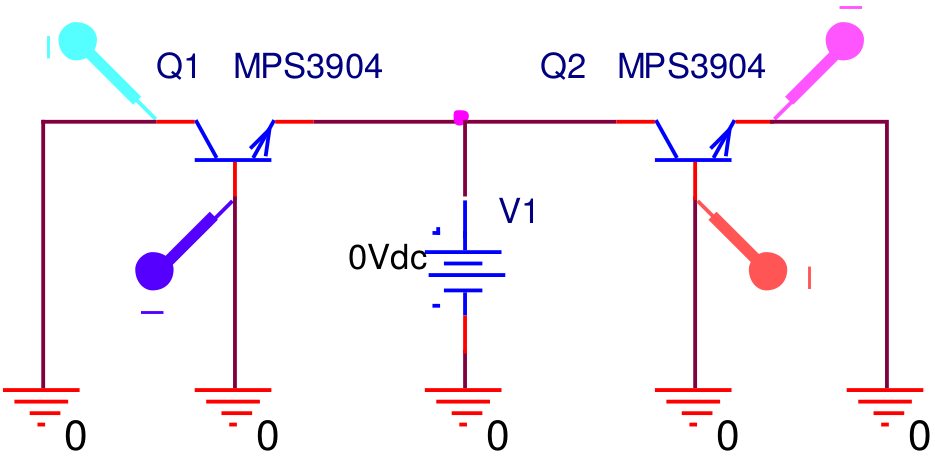
\includegraphics[width = 0.6 \textwidth]{scheme-1}
	\caption{Схема включения транзисторов для моделирования токов переноса и рекомбинации n-p-n транзистора}
	\label{scheme-1}
\end{figure}

\begin{figure}[H]
	\centering
	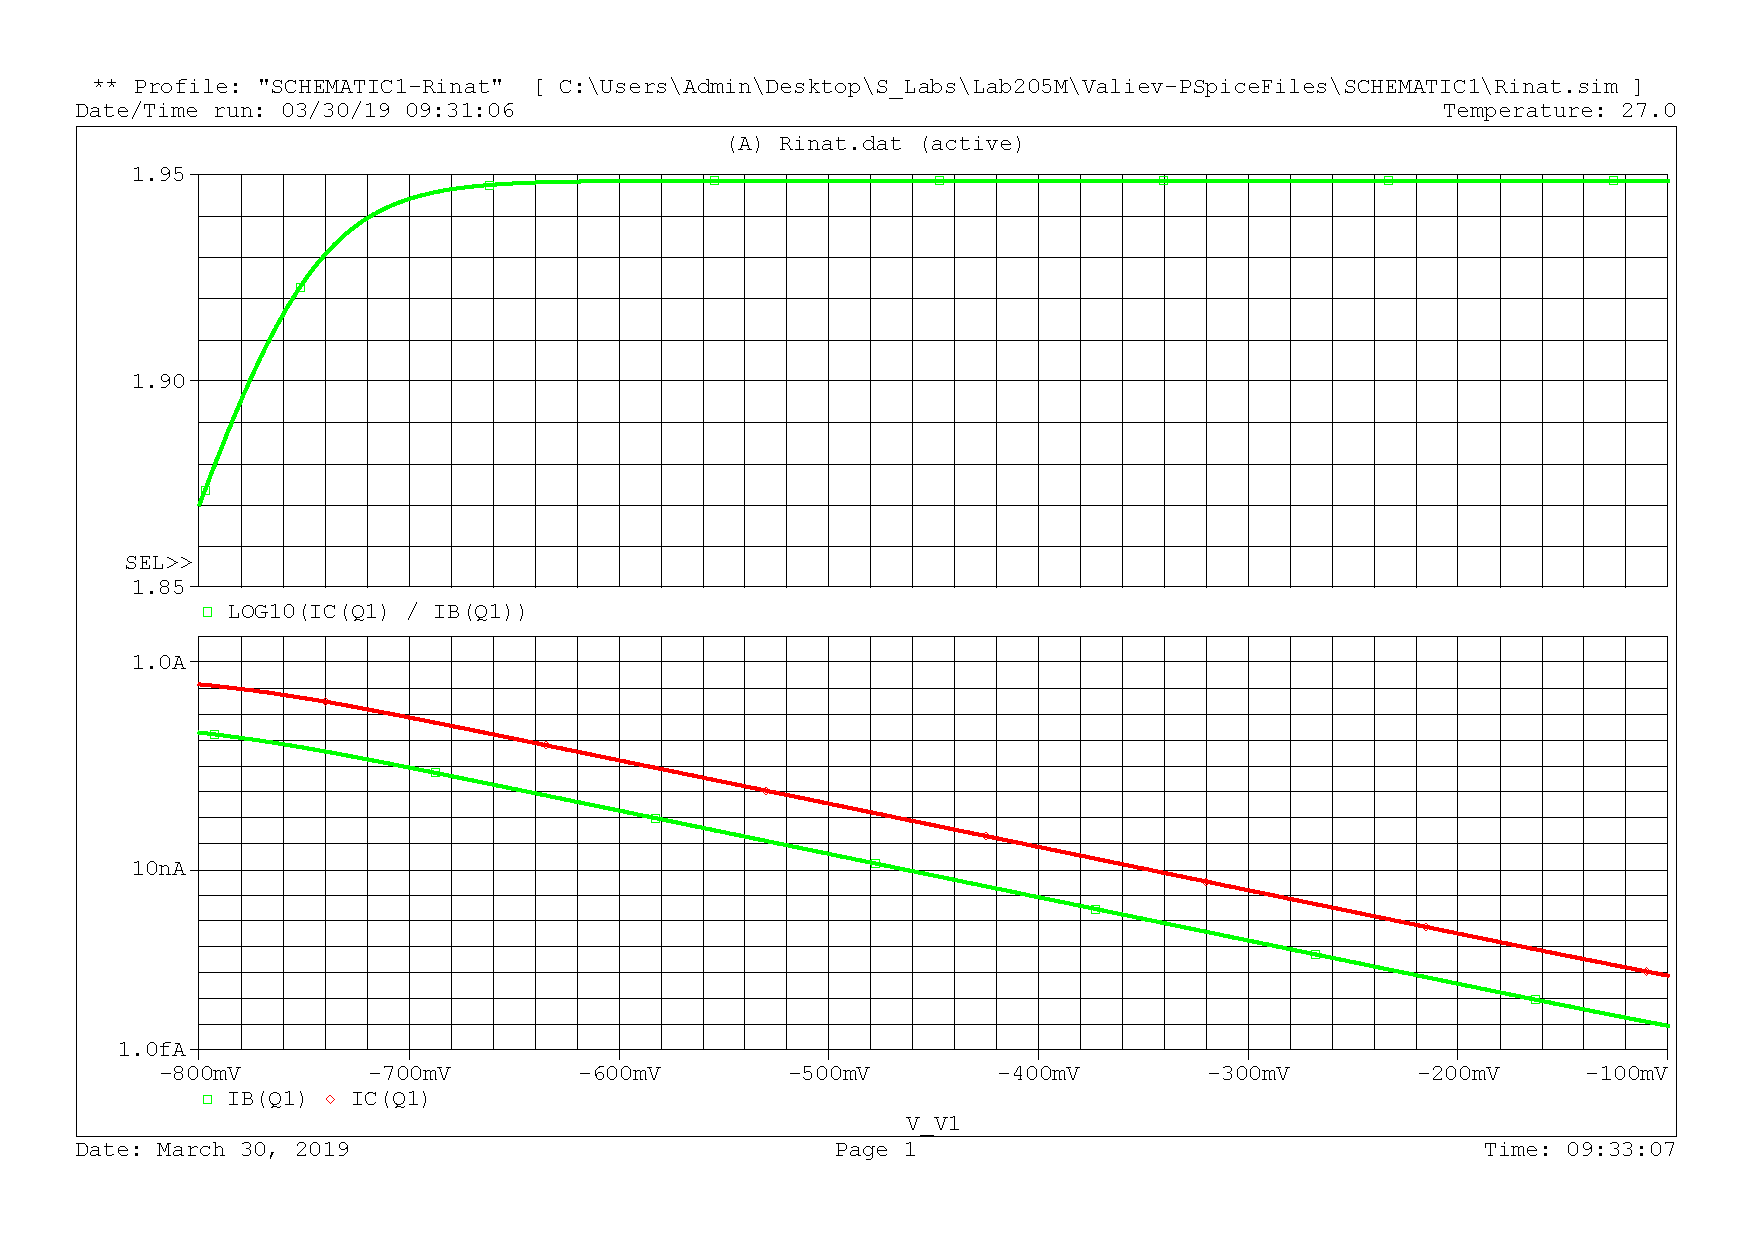
\includegraphics[width = \textwidth]{1-1}
	\caption{Прямое включение n-p-n транзистора}
\end{figure}

\begin{figure}[H]
	\centering
	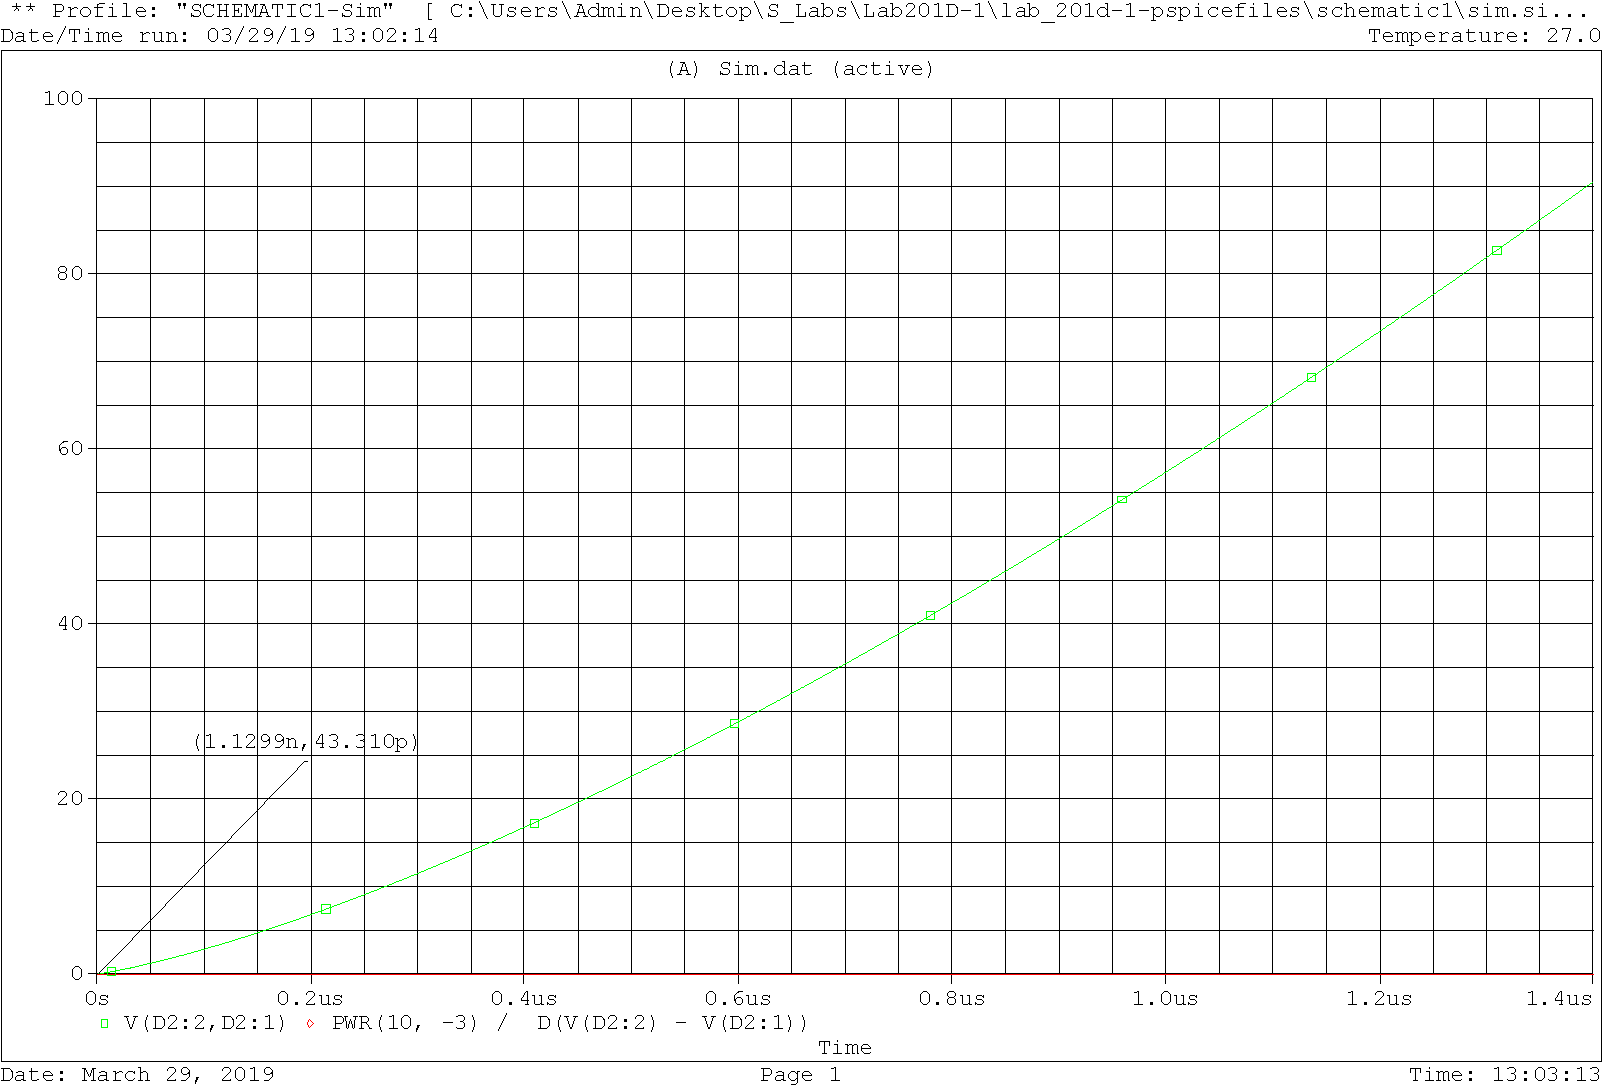
\includegraphics[width = \textwidth]{1-2}
	\caption{Инверсное включение n-p-n транзистора}
\end{figure}

\textbf{{\normalsize 2.}}
Составим схему (рис. \ref{scheme-2}). Получим зависимости токов переноса -IC(Q1) и токов рекомбинации -IB(Q1) для прямого Q1 и -IE(Q2), -IB(Q2) инверсного Q2 включения p-n-p транзистора от напряжения источника V1. Приведем графики полученных зависимостей в логарифмическом масштабе, также приведем графики десятичных логарифмов отношения токов переноса к токам рекомбинации $ \log_{10} ( \text{IC(Q1)} / \text{IB(Q1)} ) $ и $ \log_{10} ( \text{IE(Q2)} / \text{IB(Q2)} ) $.

\begin{figure}[H]
	\centering
	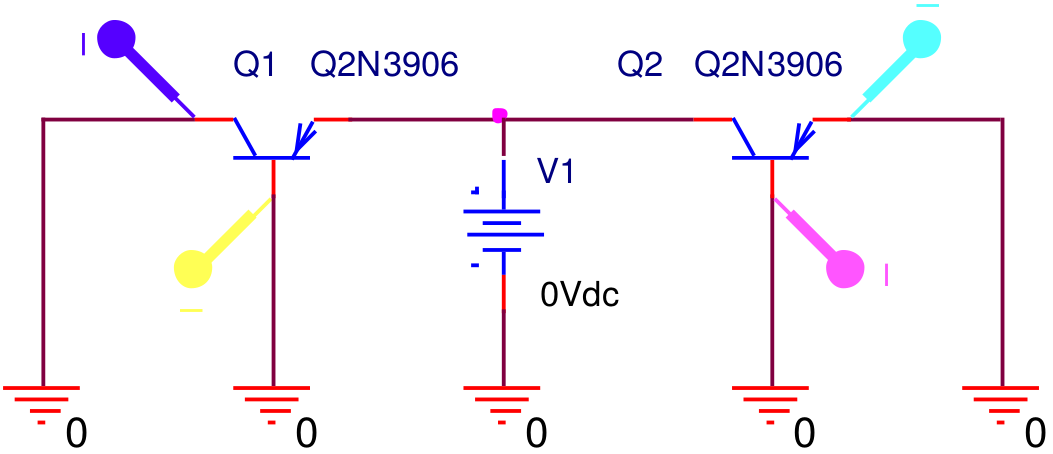
\includegraphics[width = 0.7 \textwidth]{scheme-2}
	\caption{Схема включения транзисторов для моделирования токов переноса и рекомбинации p-n-p транзистора}
	\label{scheme-2}
\end{figure}

\begin{figure}[H]
	\centering
	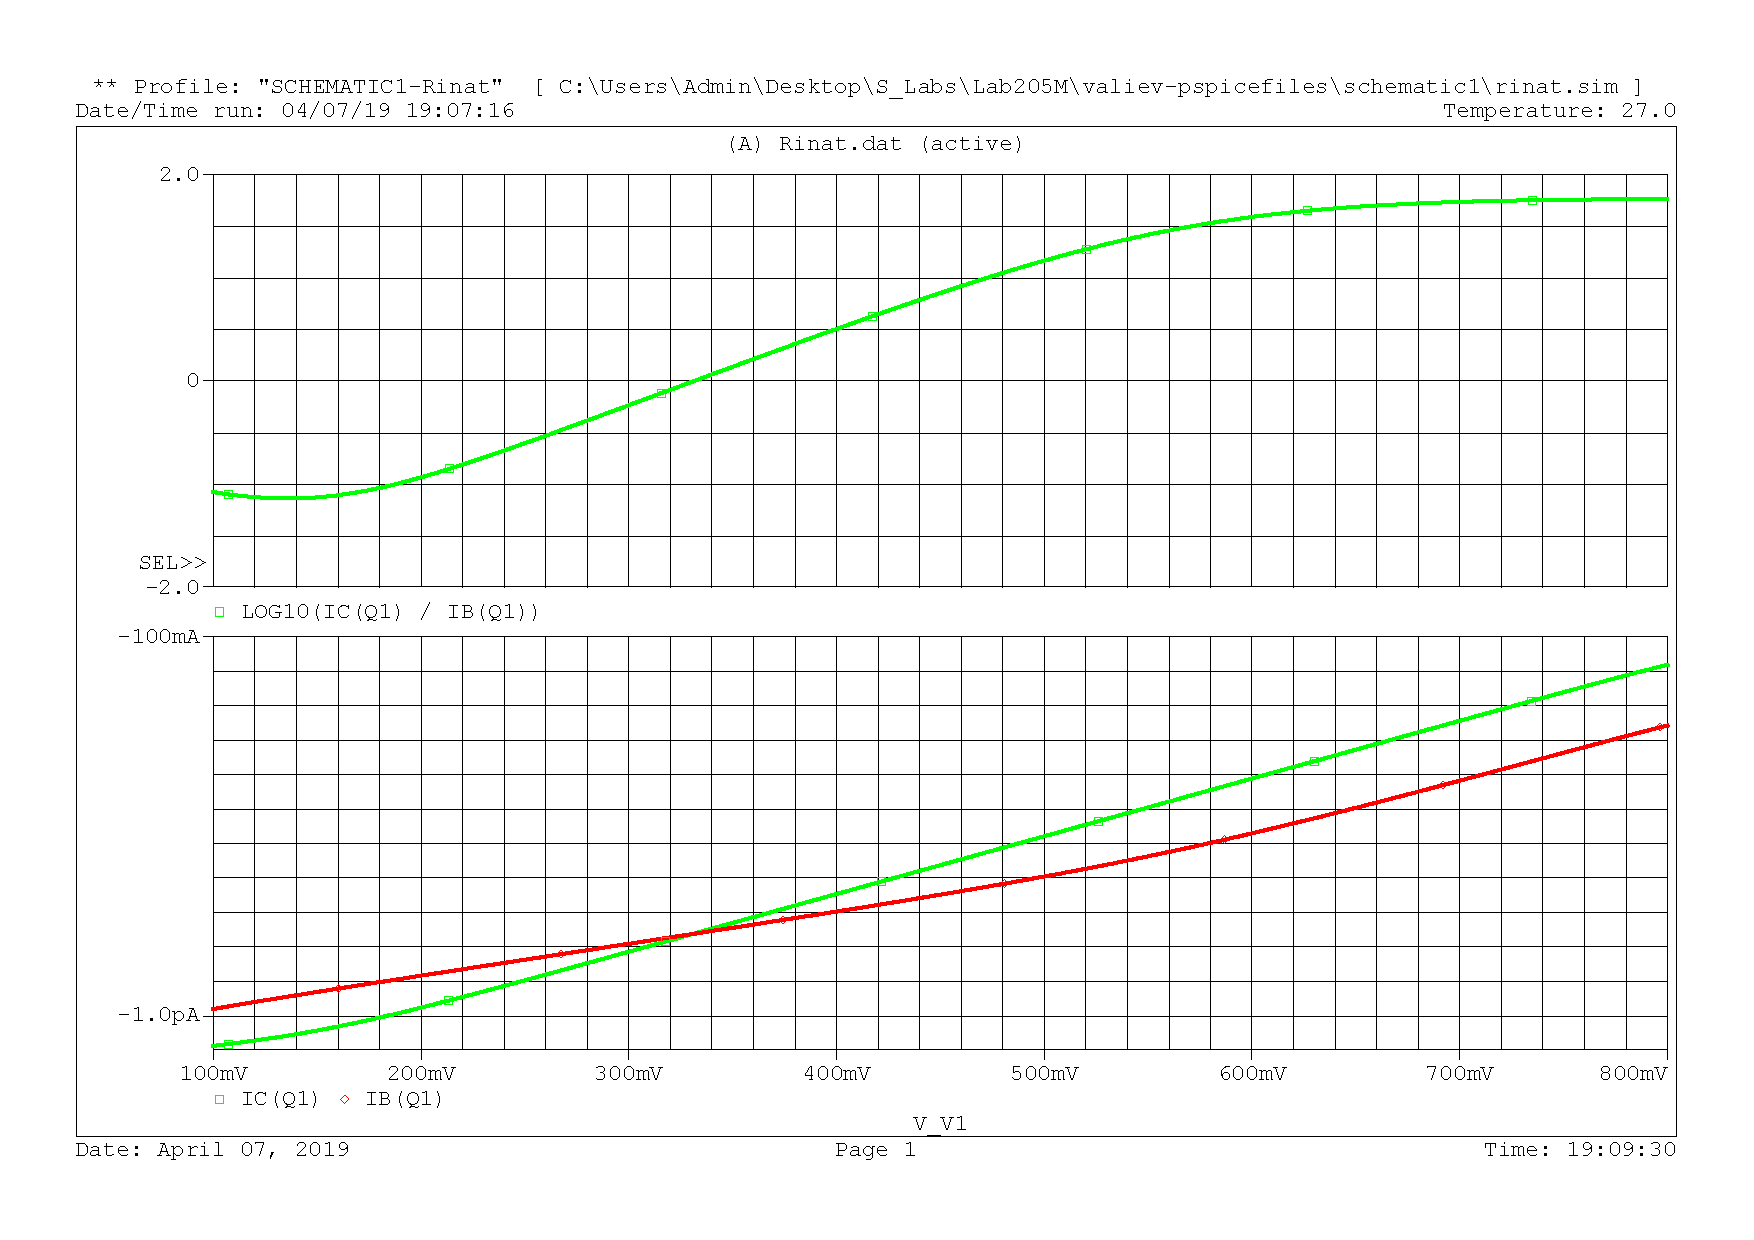
\includegraphics[width = \textwidth]{2-1}
	\caption{Прямое включение p-n-p транзистора}
\end{figure}

\begin{figure}[H]
	\centering
	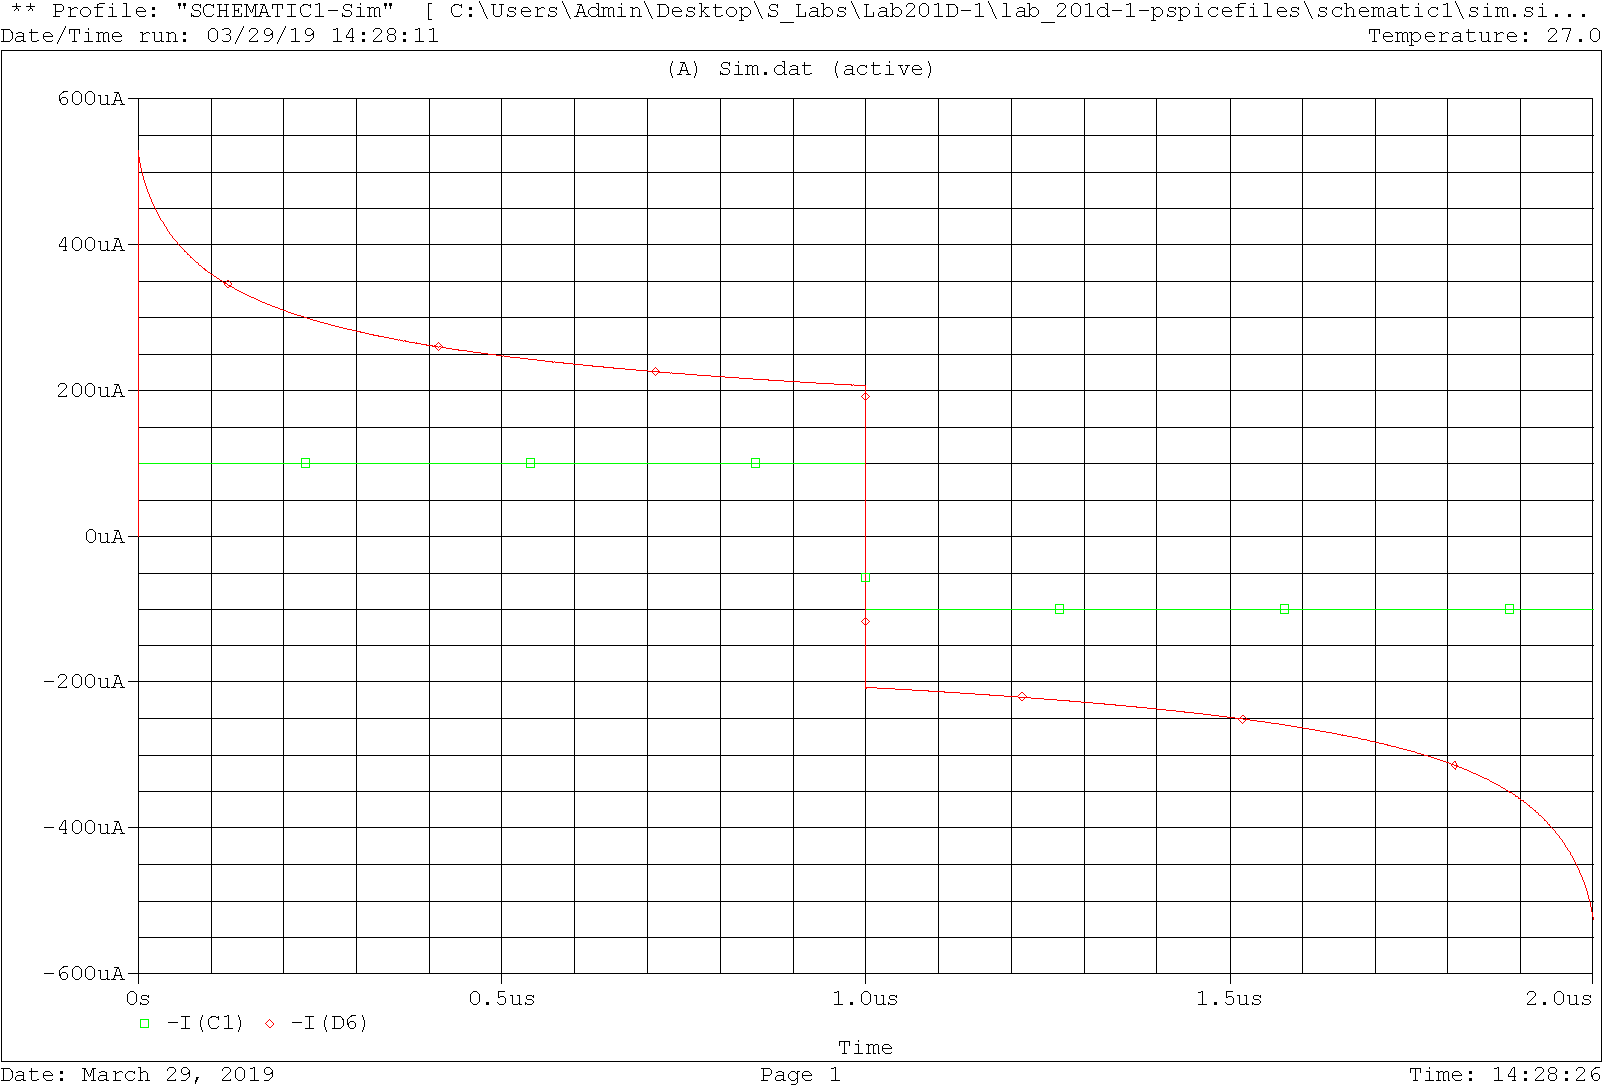
\includegraphics[width = \textwidth]{2-2}
	\caption{Инверсное включение p-n-p транзистора}
\end{figure}

\textbf{{\normalsize 3.}}
Составим схему (рис. \ref{scheme-3}). Установим ток источника тока I1 равным 1mA, напряжение источника напряжения V1 оставим равным 0VDc, установим пробник напряжения на цепь эмиттера Q1, проведем сканирование по V1 в диапазоне от -0.7V до +1V, измерим напряжение V(Q1:e) на эмиттере Q1 при V1=0. Установим на источнике V2 это напряжение. В результате этого токи эмиттеров обоих транзисторов при V1=0 будут одинаковыми.

Получим токи коллектора обоих транзисторов от V1.
Повторим при трех значениях температуры: 17, 27, 37.

Для транзистора Q1 получим зависимость тока коллектора от V1 при значениях тока эмиттера: 0, 1mA, 2mA, 3mA, 4mA.

\begin{figure}[H]
	\centering
	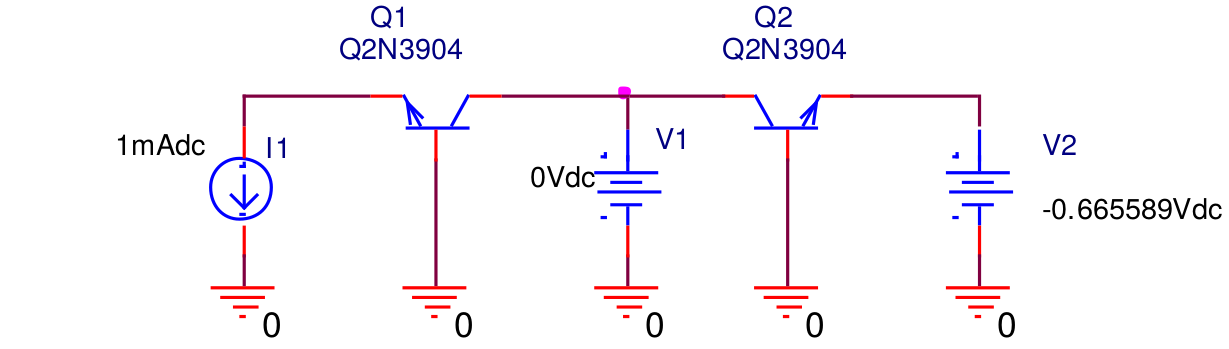
\includegraphics[width = \textwidth]{scheme-3}
	\caption{Схема моделирования выходных вольт-амперных характеристик n-p-n транзистора в схеме с общей базой}
	\label{scheme-3}
\end{figure}

\begin{figure}[H]
	\centering
	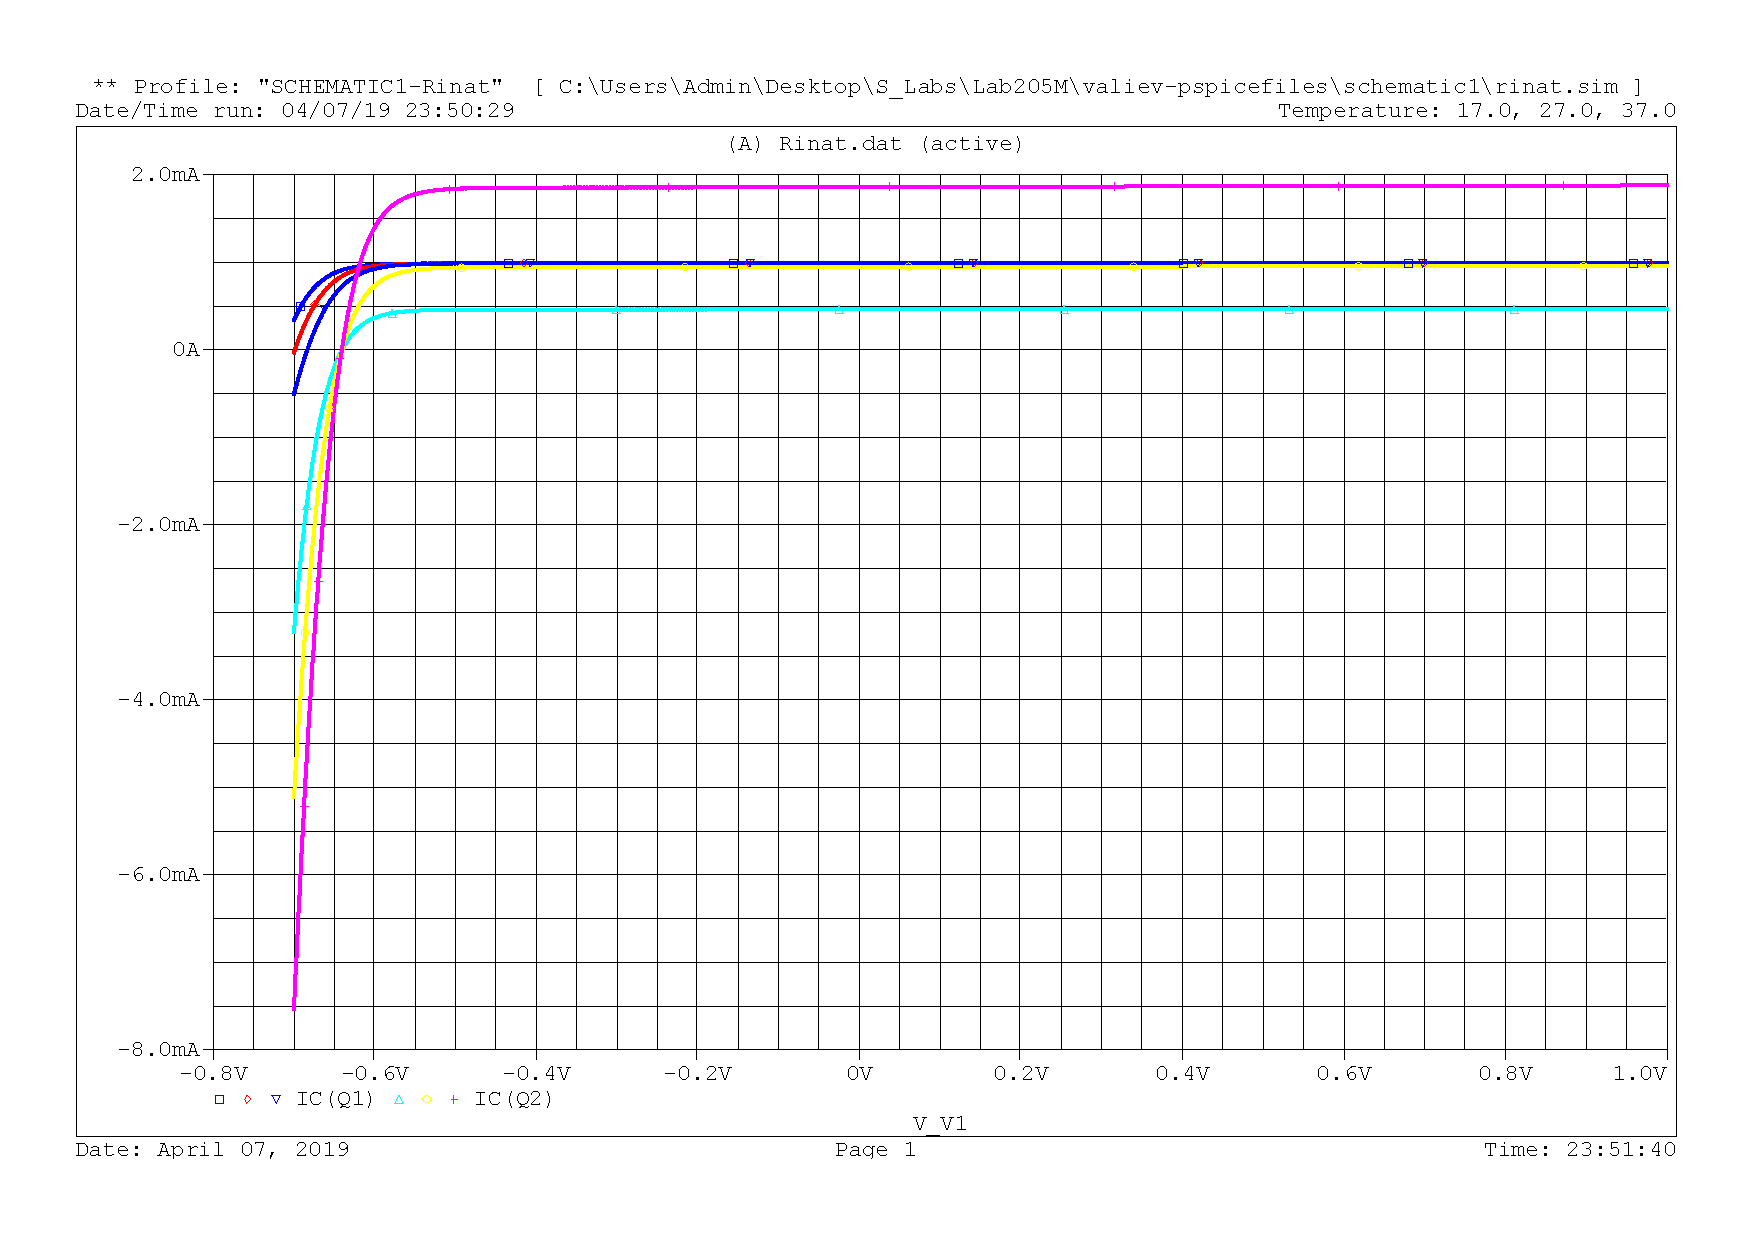
\includegraphics[width = \textwidth]{3-1}
	\caption{Ток коллектора для обоих транзисторов при разных температурах}
\end{figure}

\begin{figure}[H]
	\centering
	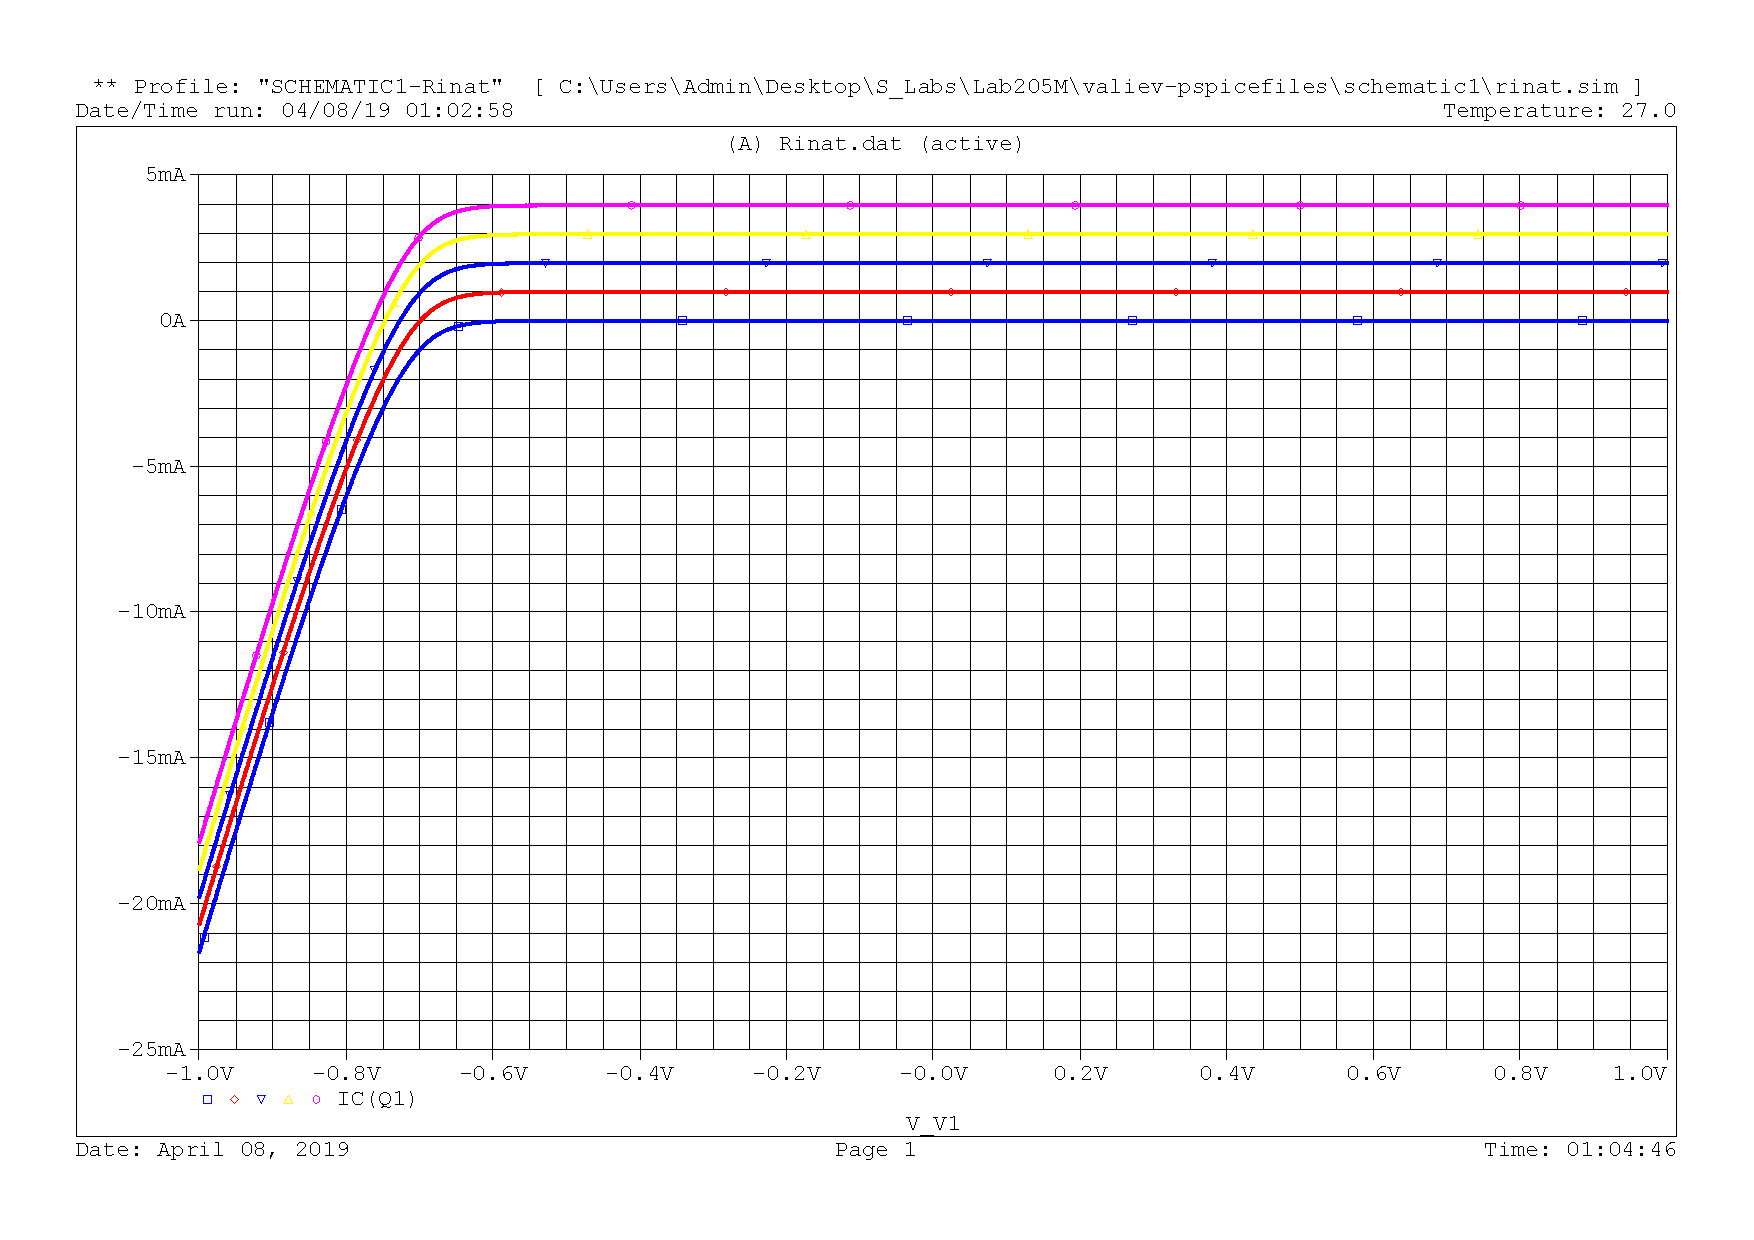
\includegraphics[width = \textwidth]{3-2}
	\caption{Зависимость тока коллектора Q1 от V1 при разных значениях тока эмиттера}
\end{figure}

\textbf{{\normalsize 4.}}
Составим схему (рис. \ref{scheme-4}). Установим (аналогично предыдущему пункту) на источнике V2 такое напряжение, чтобы токи эмиттеров обоих транзисторов при V1=0 были равными 1mA.

Получим токи коллектора обоих транзисторов от V1.
Повторим при трех значениях температуры: 17, 27, 37.

Для транзистора Q1 получим зависимость тока коллектора от V1 при значениях тока эмиттера: 0, 1mA, 2mA, 3mA, 4mA.

\begin{figure}[H]
	\centering
	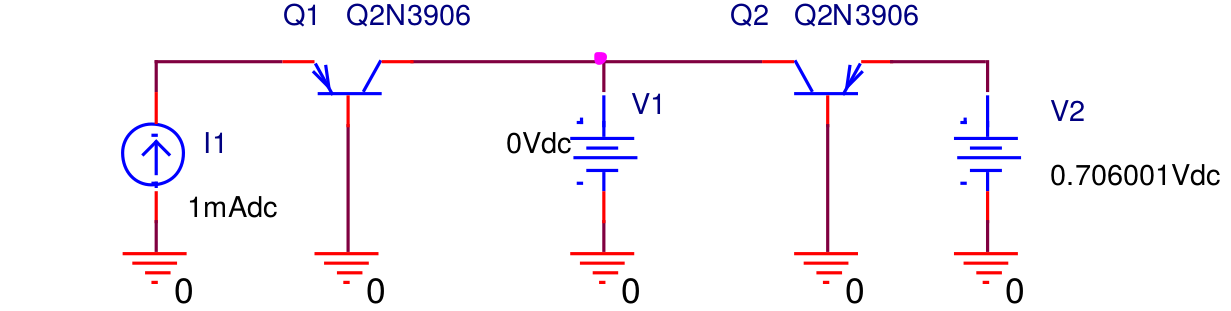
\includegraphics[width = \textwidth]{scheme-4}
	\caption{Схема моделирования выходных вольт-амперных характеристик p-n-p транзистора в схеме с общей базой}
	\label{scheme-4}
\end{figure}

\begin{figure}[H]
	\centering
	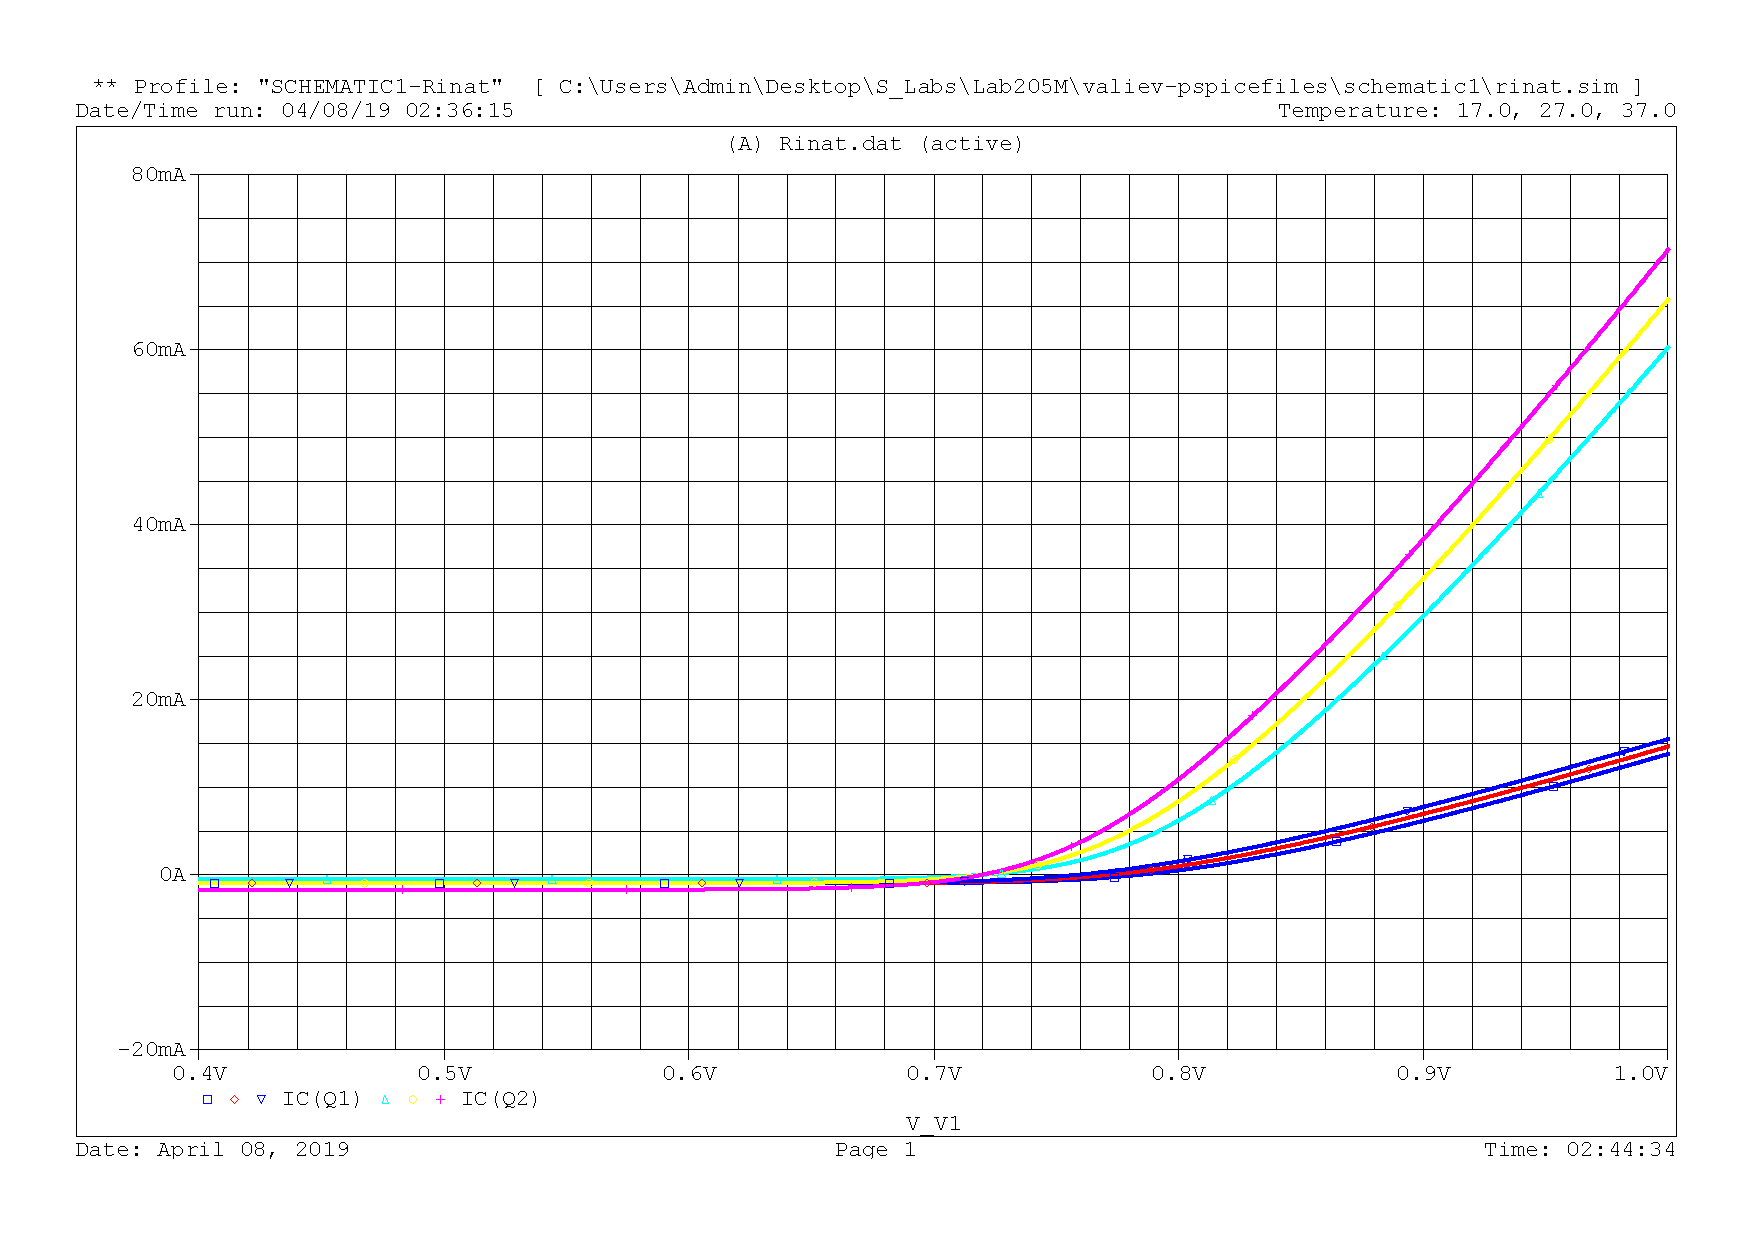
\includegraphics[width = \textwidth]{4-1}
	\caption{Ток коллектора для обоих транзисторов при разных температурах}
\end{figure}

\begin{figure}[H]
	\centering
	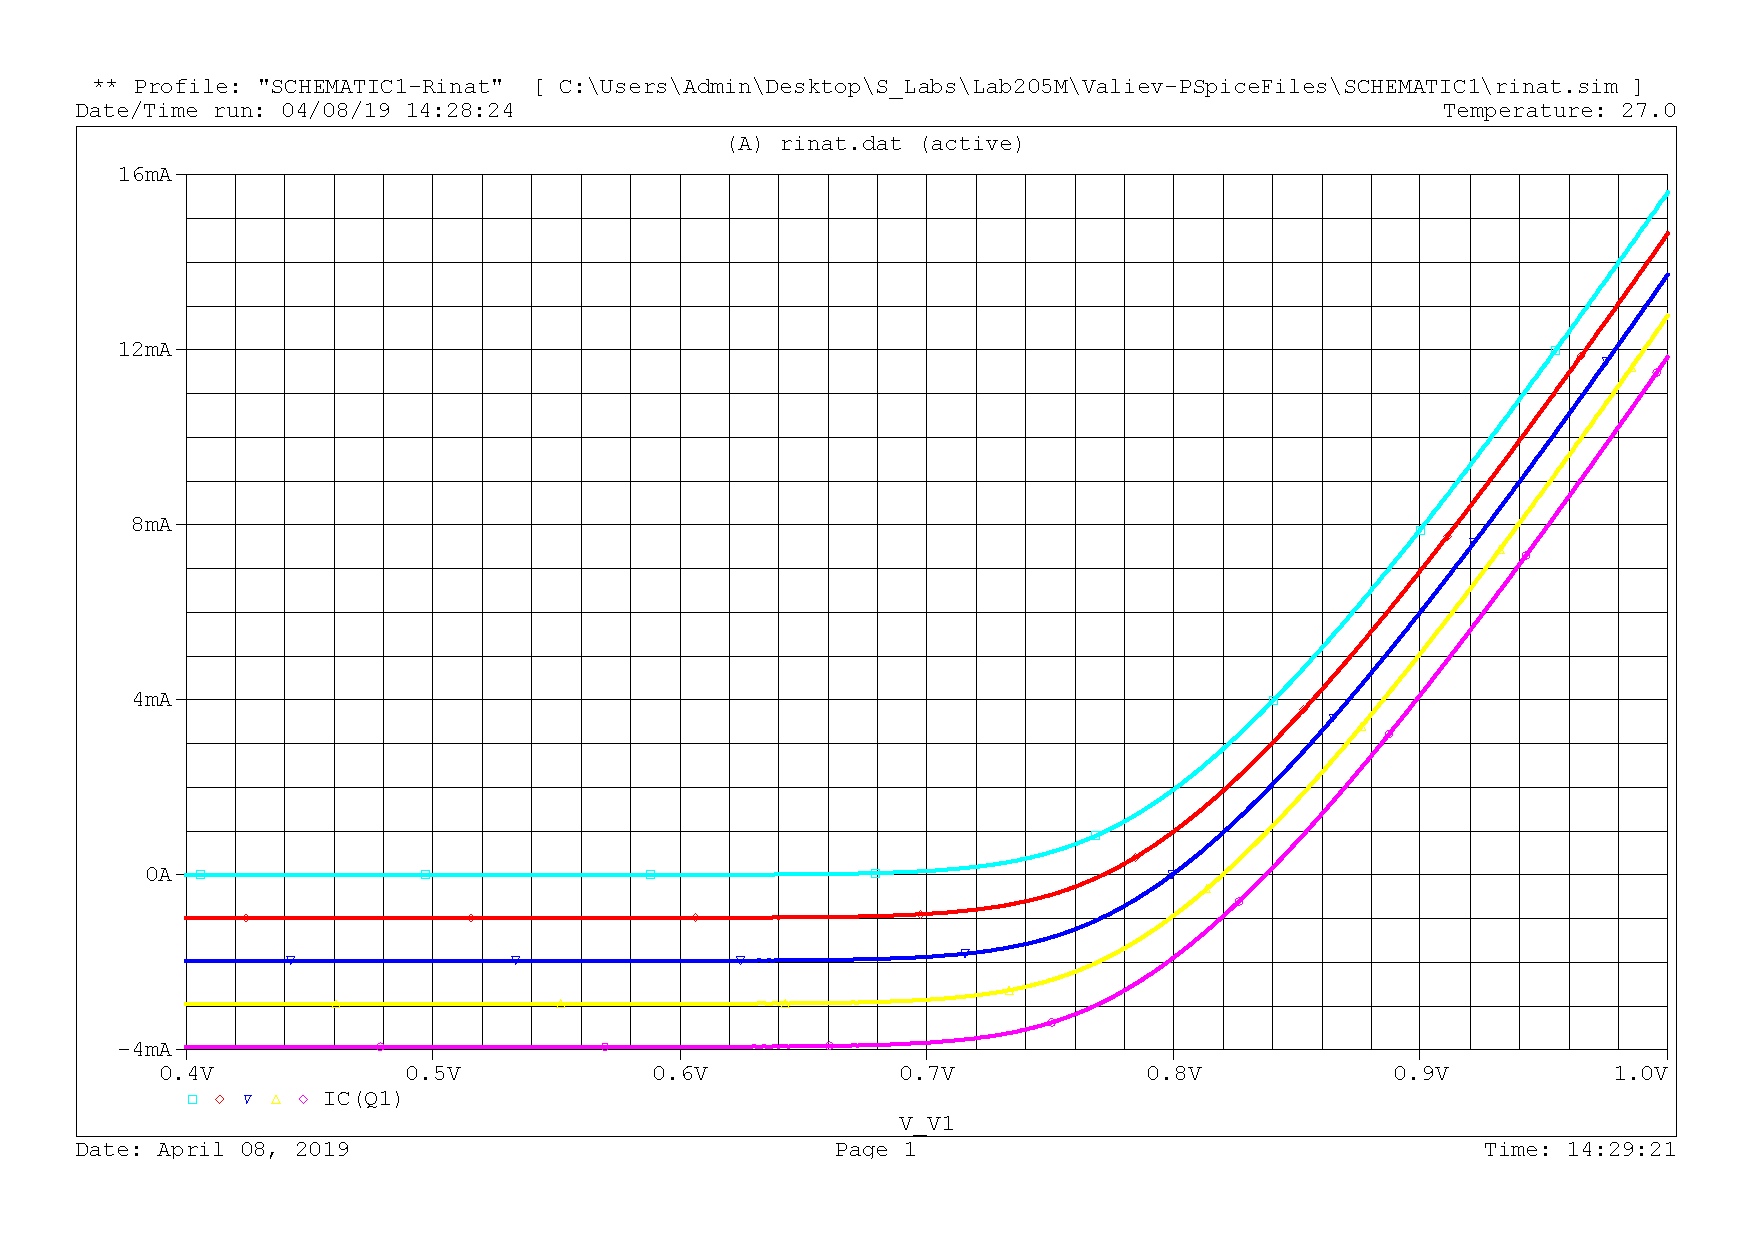
\includegraphics[width = \textwidth]{4-2}
	\caption{Зависимость тока коллектора Q1 от V1 при разных значениях тока эмиттера}
\end{figure}

\textbf{{\normalsize 5.}}
Составим схему (рис. \ref{scheme-5}). Установим напряжение источника V2 равным 0.65V-0.75V так, чтобы при сканировании по V1 от 0V до +1.0V ток коллектора Q2 при V1= +1V был в интервале от 1mA до 10mA. Измерим ток базы Q2 при V1=+1V и установим это значение тока для источника I1.

Получим токи коллектора обоих транзисторов от V1.

Исключим из схемы транзистор Q2 и получим зависимости тока коллектора Q1 от напряжения V1 для нескольких значений параметра I1: 2uA, 4uA, 6uA, 8uA, 10uA.

При фиксированном токе базы получим зависимости тока коллектора Q1 от напряжения V1 для трёх значений температуры: -40, 27 и 85 градусов.

\begin{figure}[H]
	\centering
	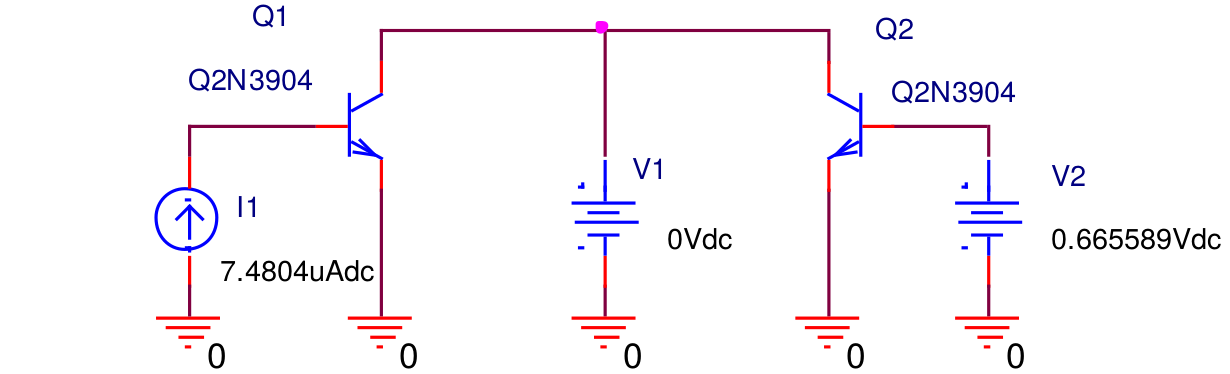
\includegraphics[width = \textwidth]{scheme-5}
	\caption{Схема моделирования выходных вольт-амперных характеристик n-p-n транзистора в схеме с общим эмиттером}
	\label{scheme-5}
\end{figure}

\begin{figure}[H]
	\centering
	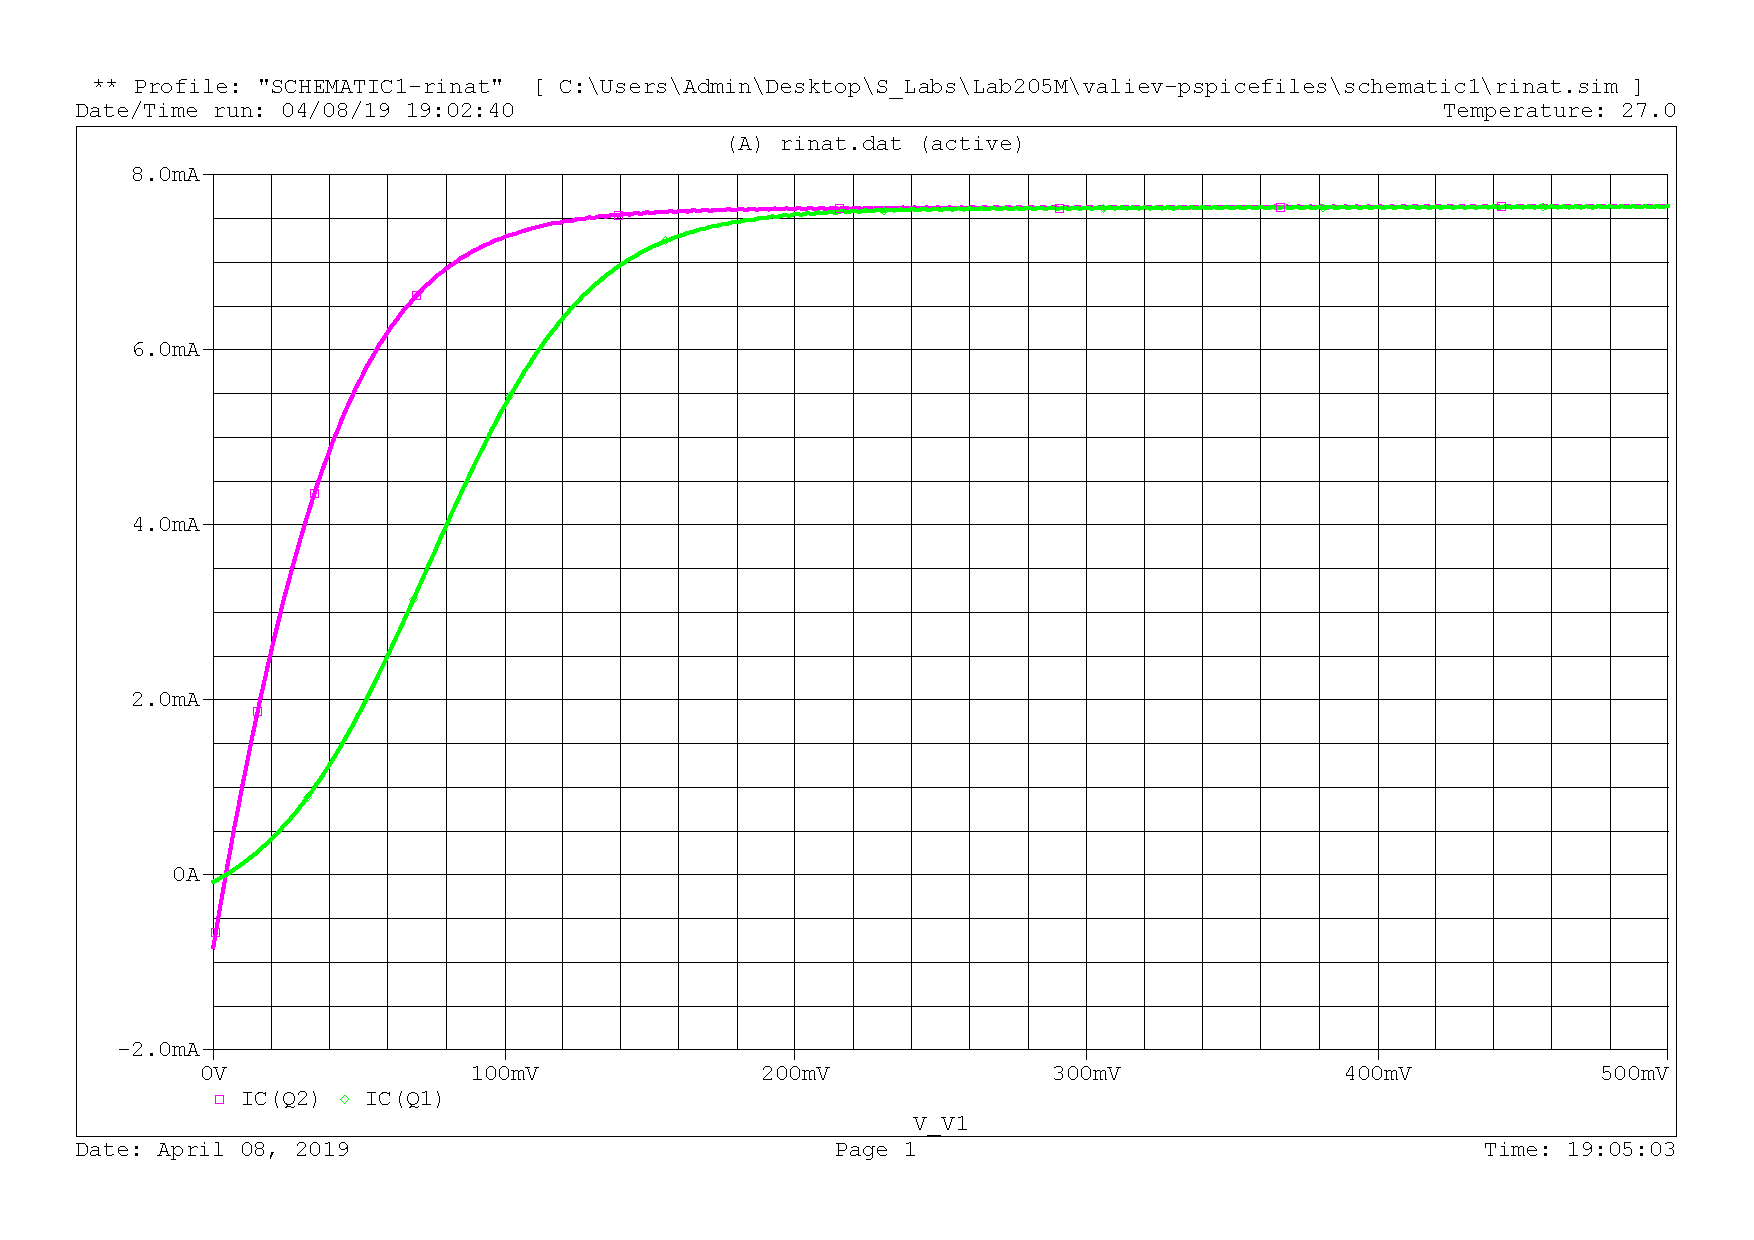
\includegraphics[width = \textwidth]{5-1}
	\caption{Ток коллектора для обоих транзисторов}
\end{figure}

\begin{figure}[H]
	\centering
	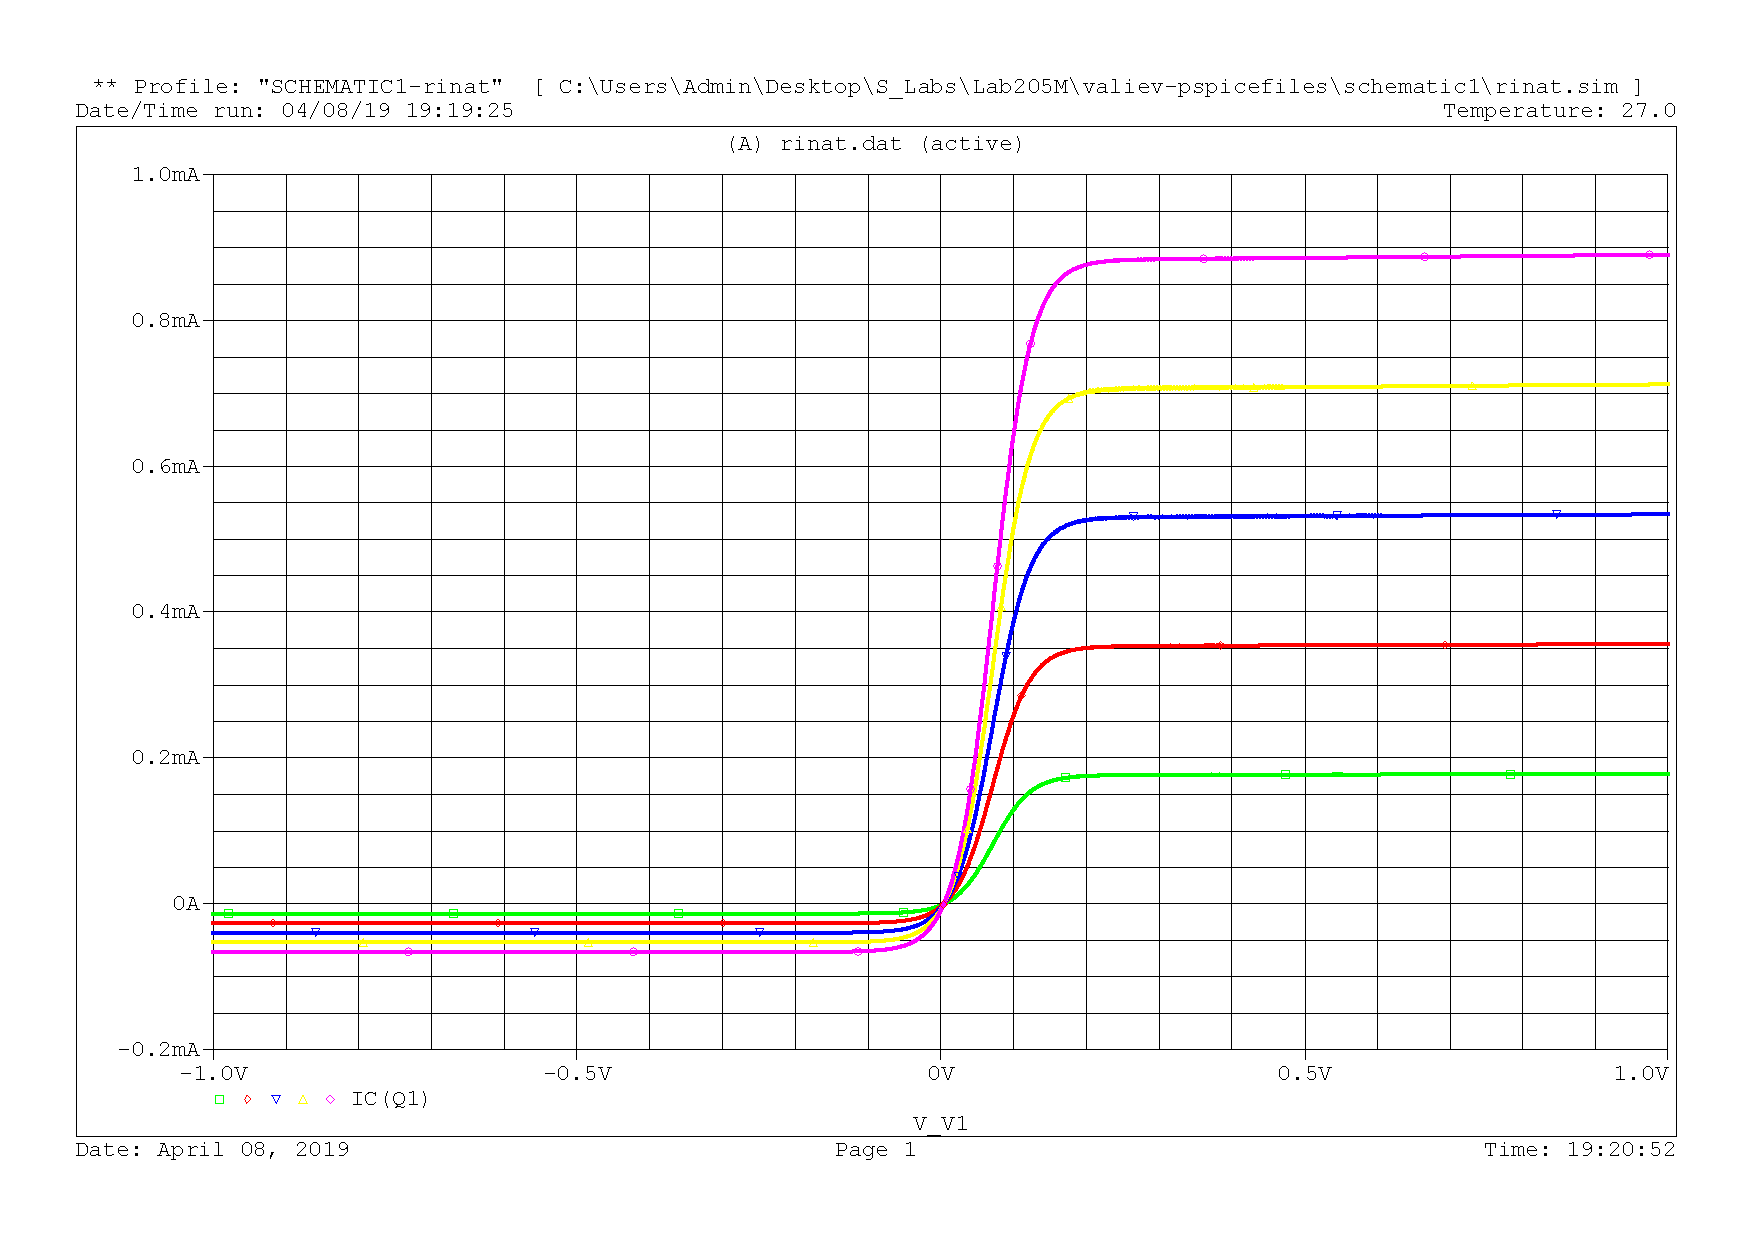
\includegraphics[width = \textwidth]{5-2}
	\caption{Ток коллектора для Q1 при разных значениях параметра I1}
\end{figure}

\begin{figure}[H]
	\centering
	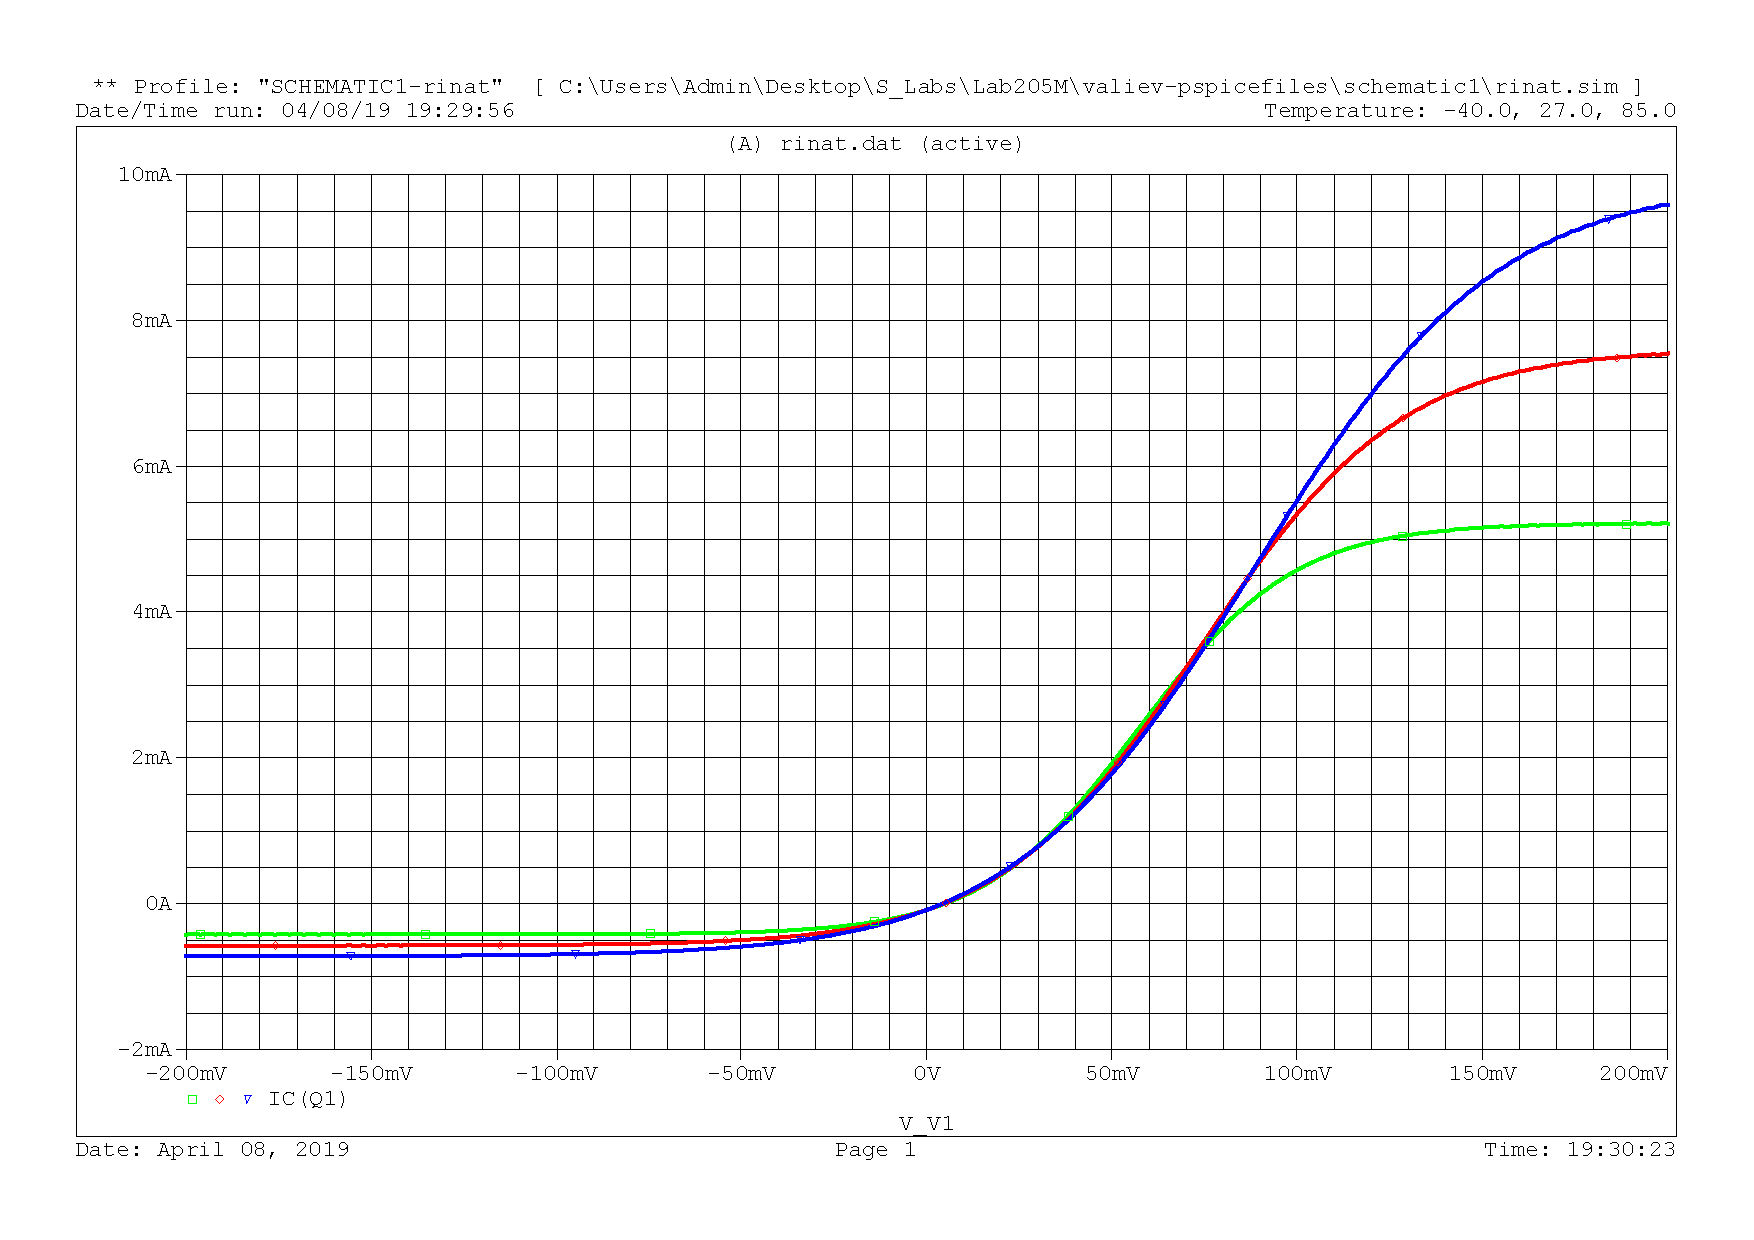
\includegraphics[width = \textwidth]{5-3}
	\caption{Ток коллектора для Q1 при разных температурах}
\end{figure}

\textbf{{\normalsize 6.}}
Составим схему (рис. \ref{scheme-6}). Установим напряжение источника V2 таким, чтобы при сканировании по V1 от -1V до 0V ток коллектора Q2 при V1=-1V был в интервале от 1mA до 10mA. Измерим ток базы Q2 при V1=-1V и установим это значение тока для источника I1.

Получим токи коллектора обоих транзисторов от V1.

Исключим из схемы транзистор Q2 и получим зависимости тока коллектора Q1 от напряжения V1 для нескольких значений параметра I1: 2uA, 4uA, 6uA, 8uA, 10uA.

При фиксированном токе базы получим зависимости тока коллектора Q1 от напряжения V1 для трёх значений температуры: -40, 27 и 85 градусов.

\begin{figure}[H]
	\centering
	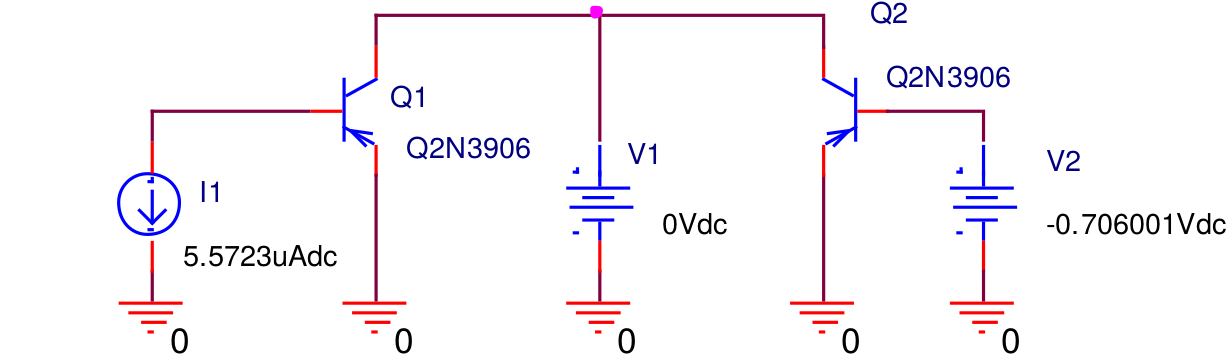
\includegraphics[width = \textwidth]{scheme-6}
	\caption{Схема моделирования выходных вольт-амперных характеристик p-n-p транзистора в схеме с общим эмиттером}
	\label{scheme-6}
\end{figure}

\begin{figure}[H]
	\centering
	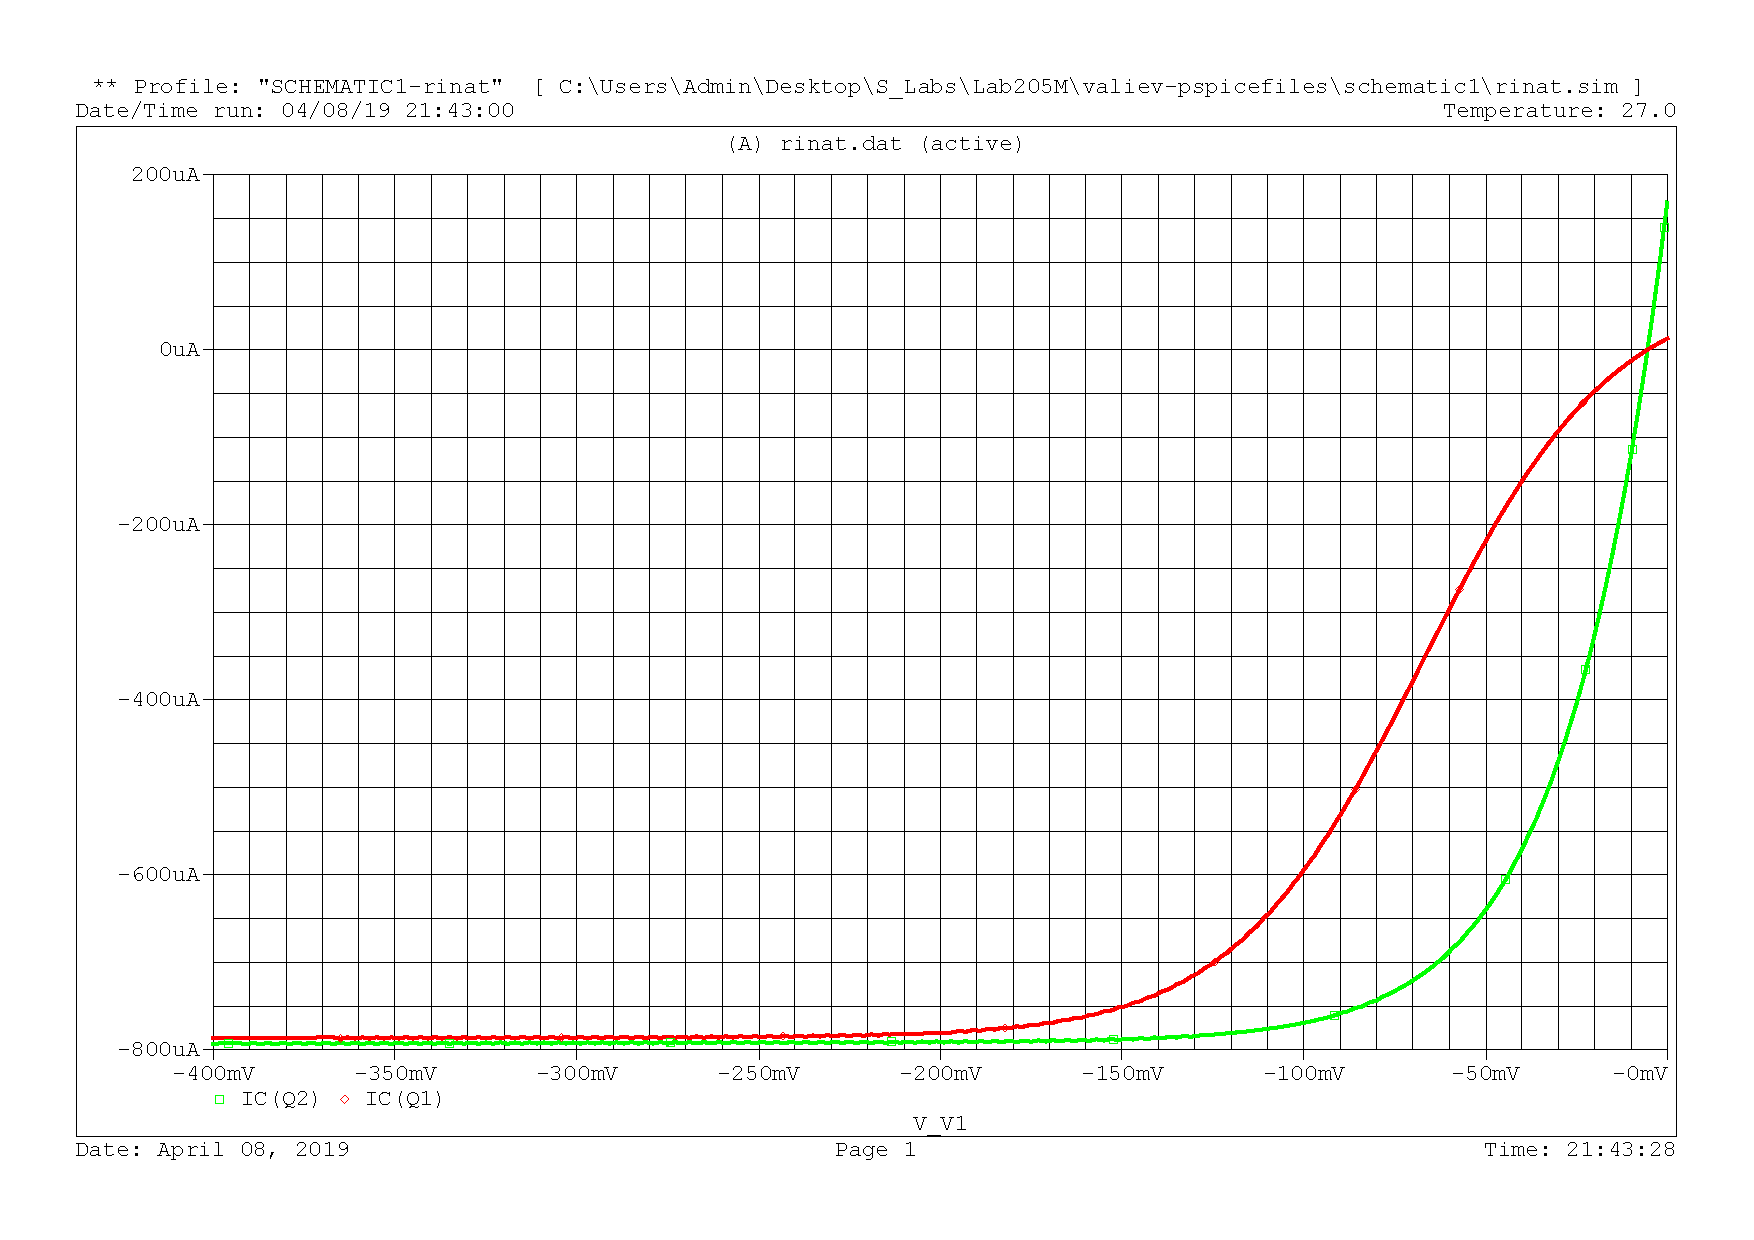
\includegraphics[width = \textwidth]{6-1}
	\caption{Ток коллектора для обоих транзисторов}
\end{figure}

\begin{figure}[H]
	\centering
	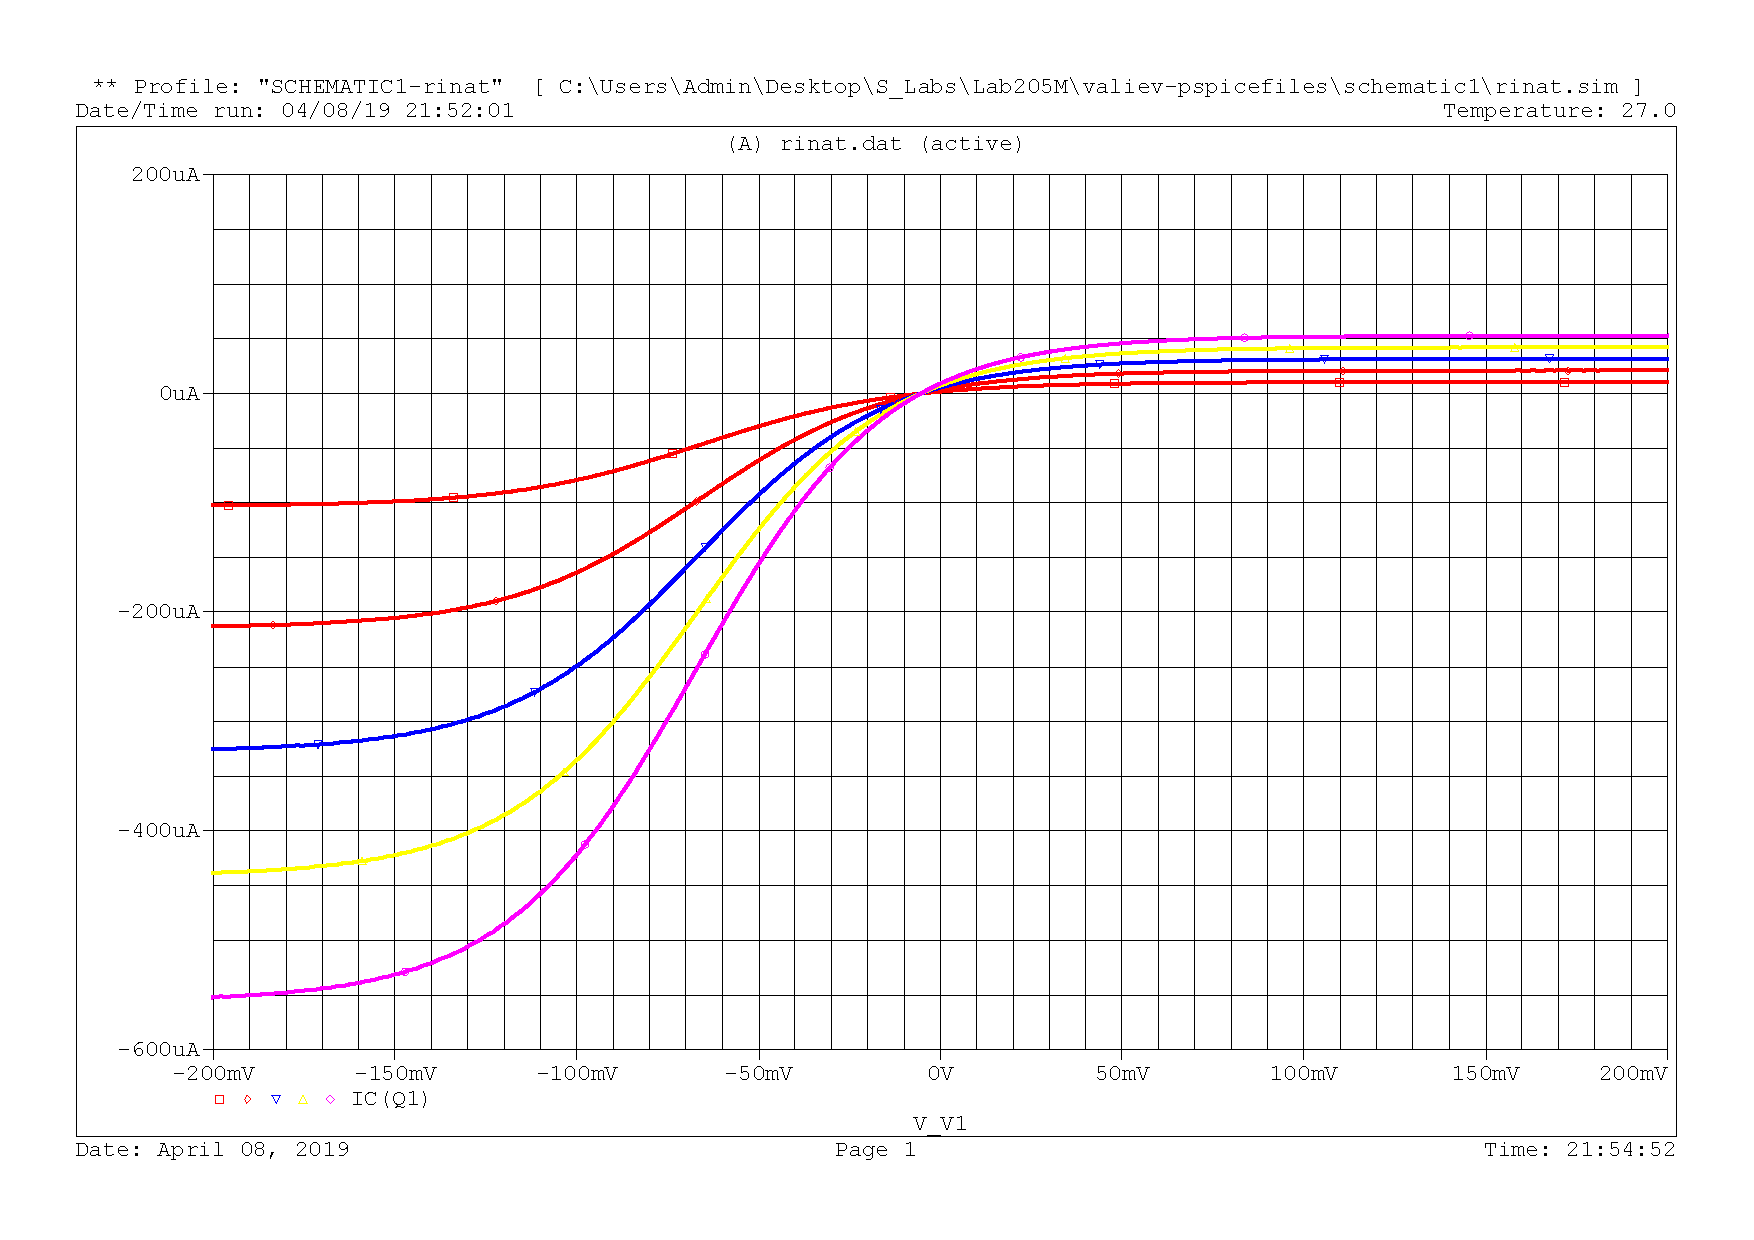
\includegraphics[width = \textwidth]{6-2}
	\caption{Ток коллектора для Q1 при разных значениях параметра I1}
\end{figure}

\begin{figure}[H]
	\centering
	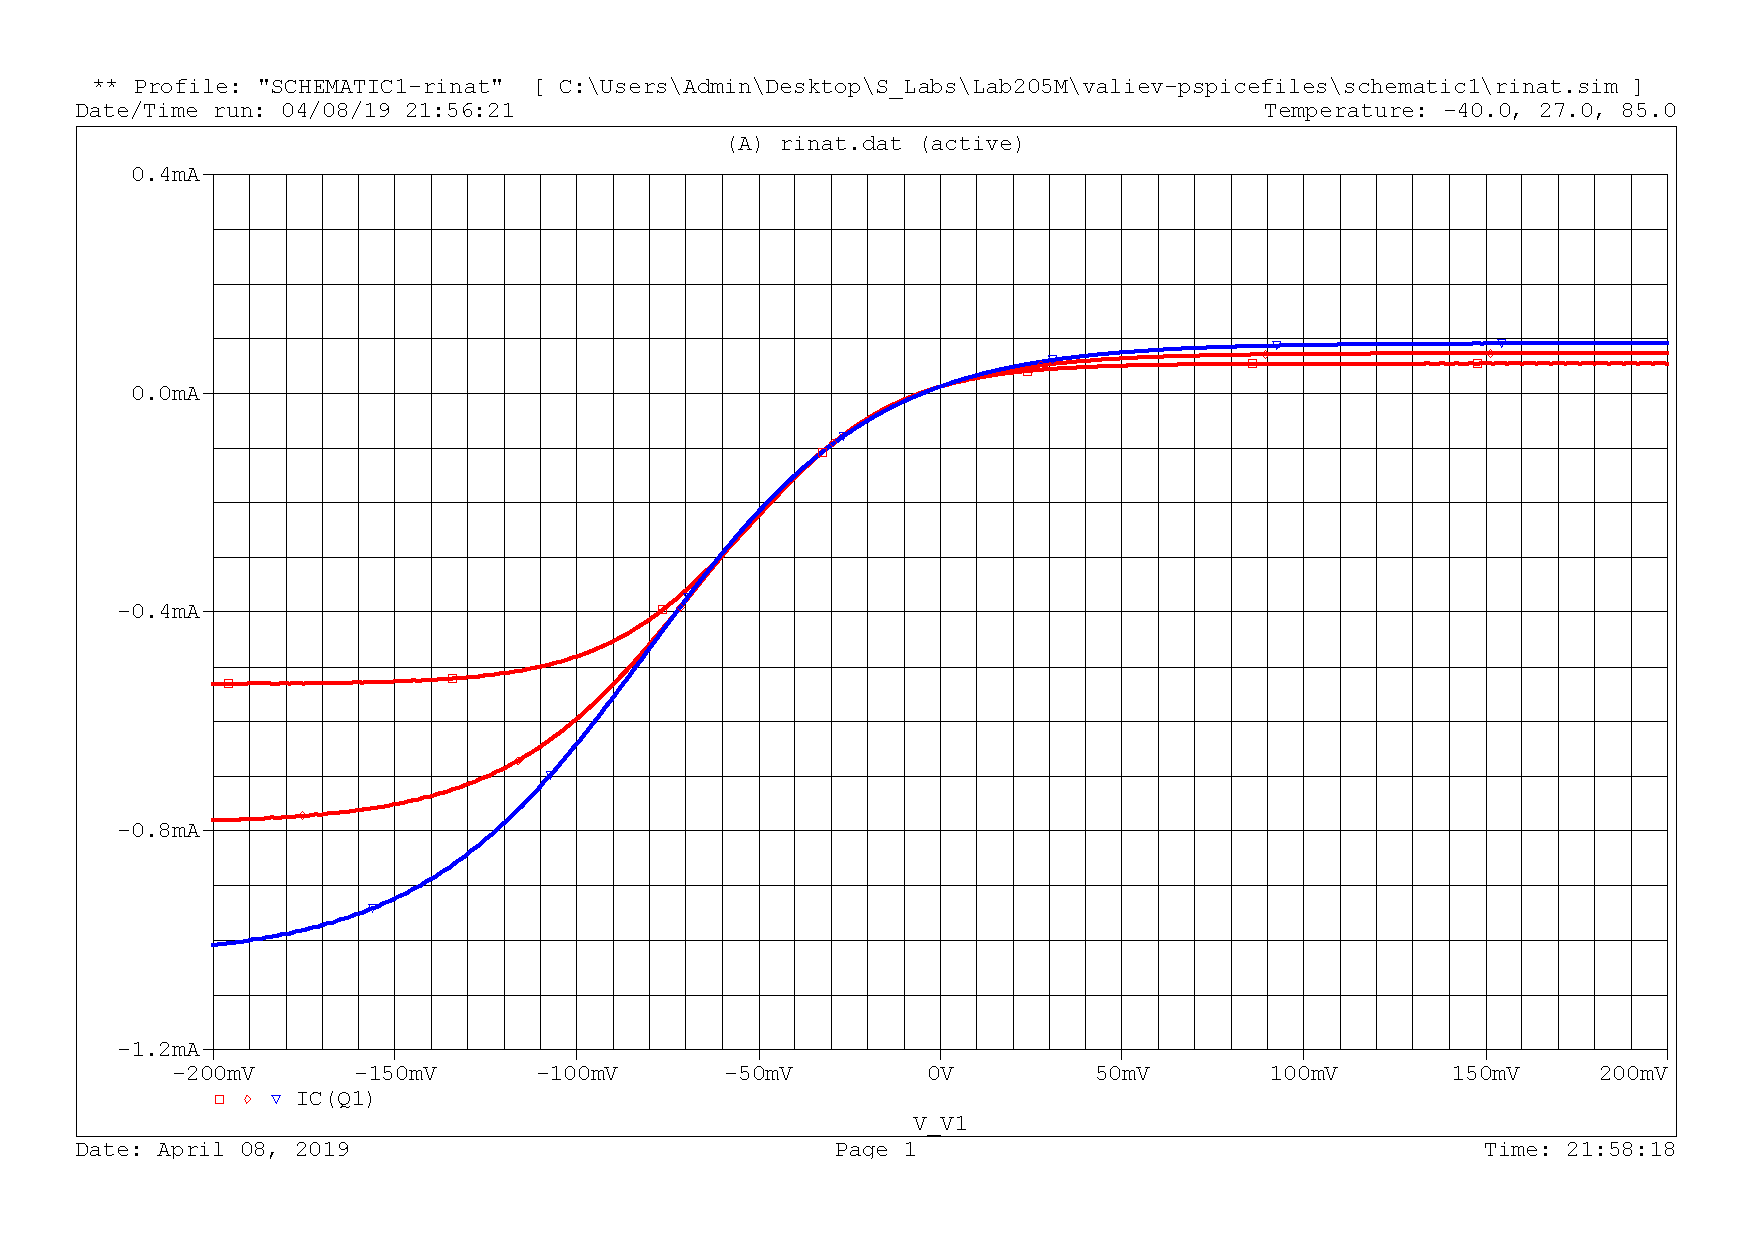
\includegraphics[width = \textwidth]{6-3}
	\caption{Ток коллектора для Q1 при разных температурах}
\end{figure}

\textbf{{\normalsize 7.}}
Составим схему (рис. \ref{scheme-7}) моделирования напряжения на коллекторе транзистора в схеме с общим эмиттером при нулевом токе коллектора в зависимости от тока базы n-p-n и n-p-n транзисторов ($ \text{U}_{\text{ce}0} (\text{IB}) $)

Получим зависимости напряжений на коллекторах транзисторов от тока базы.

\begin{figure}[H]
	\centering
	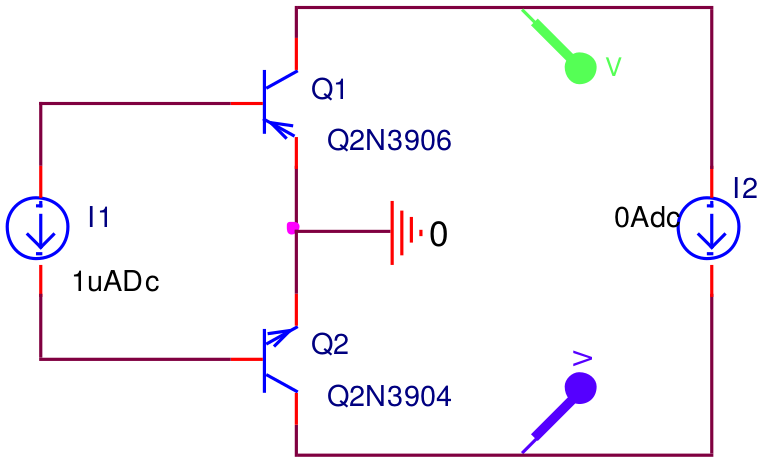
\includegraphics[width = 0.55 \textwidth]{scheme-7}
	\caption{Схема моделирования $ \text{U}_{\text{ce}0} $}
	\label{scheme-7}
\end{figure}

\begin{figure}[H]
	\centering
	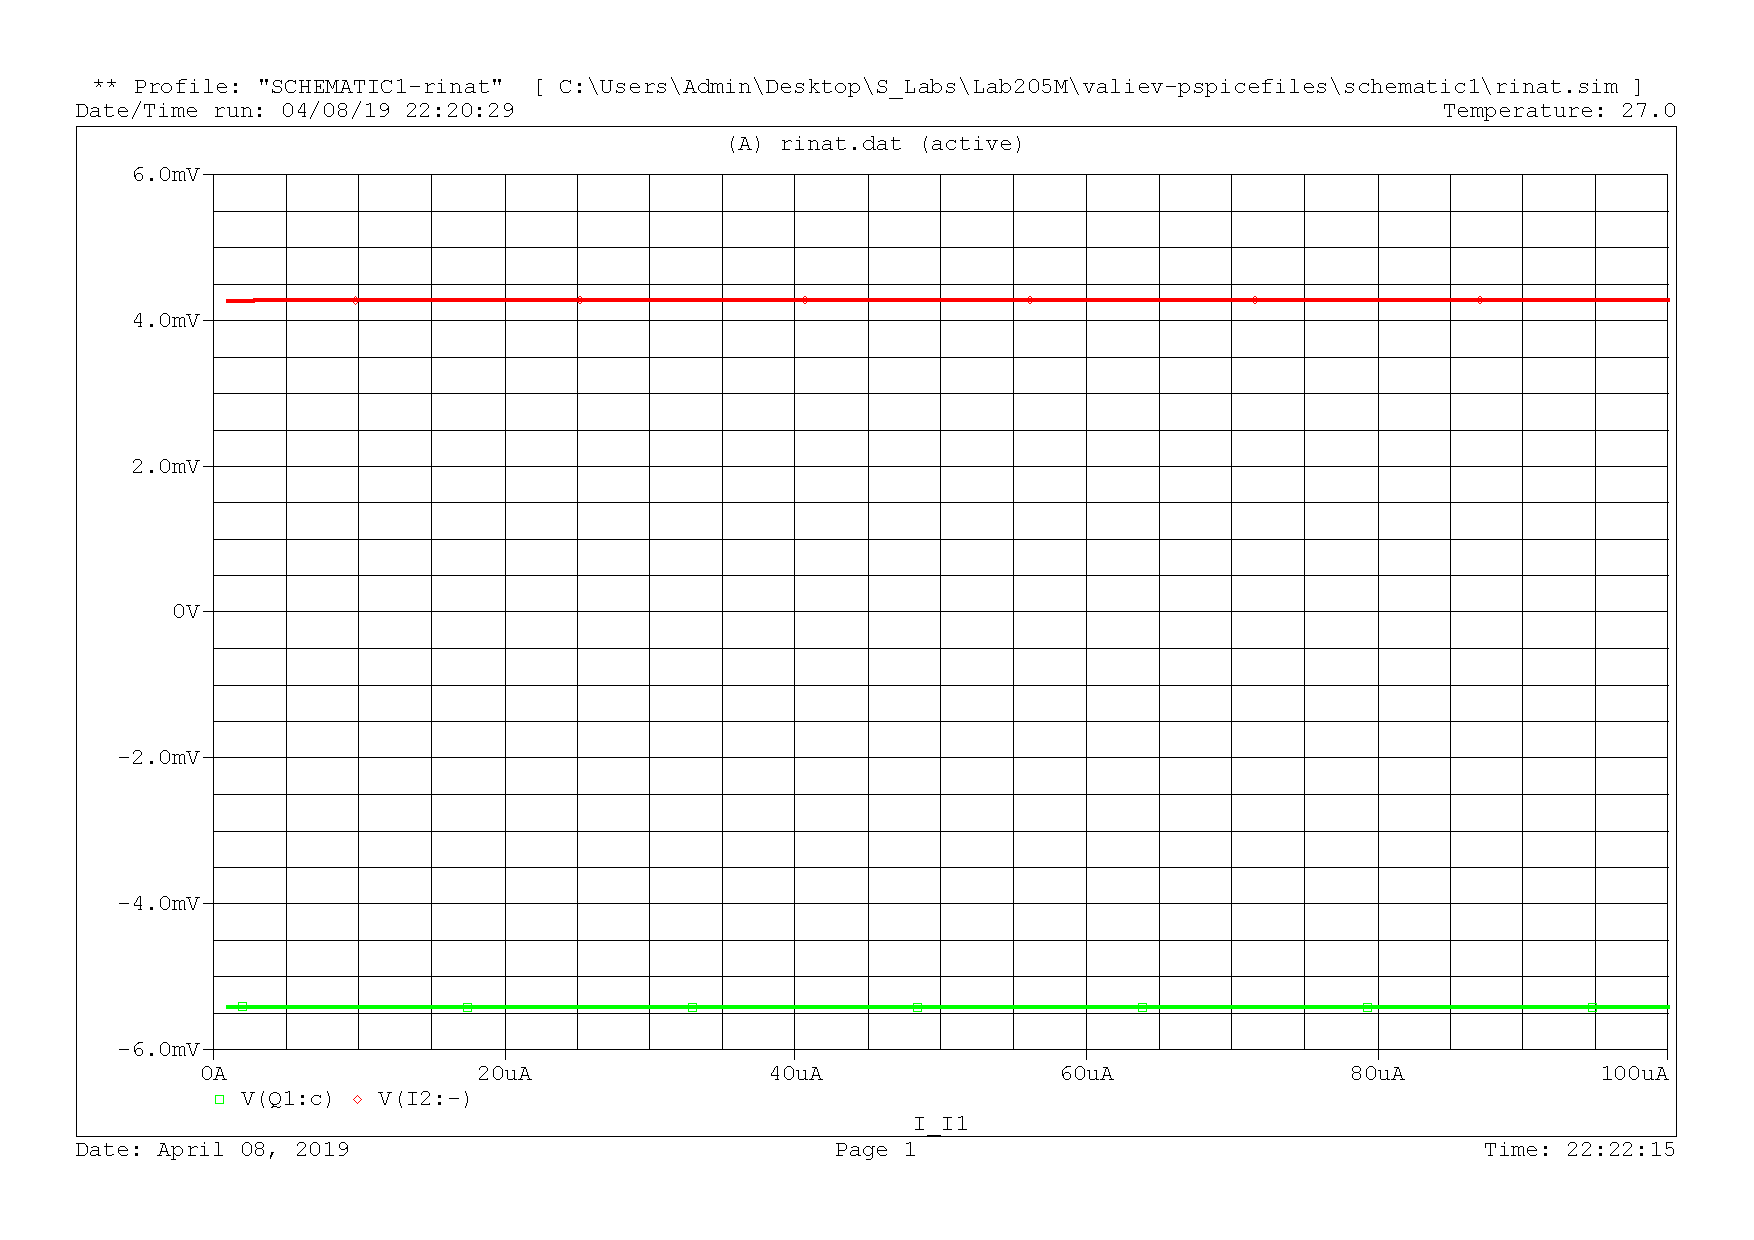
\includegraphics[width = \textwidth]{7}
	\caption{Зависимость напряжений на коллекторах транзисторов от тока базы}
\end{figure}

\end{document}